\documentclass[10pt,openany]{book}
\usepackage[utf8]{inputenc}
\DeclareUnicodeCharacter{2212}{\ensuremath{-}}
\DeclareUnicodeCharacter{2192}{\ensuremath{\to}}
\DeclareUnicodeCharacter{03B1}{\ensuremath{\alpha}}
\usepackage[T1]{fontenc}
\usepackage{lmodern}
\usepackage[spanish,es-nodecimaldot]{babel}
\spanishplainpercent
\AtBeginDocument{\spanishdeactivate{"~<>}}
\usepackage[a4paper,margin=2.5cm,headheight=14pt]{geometry}
\usepackage{amsmath,amssymb,mathtools,booktabs,array,longtable,graphicx,xcolor,tikz,enumitem,microtype,titlesec,fancyhdr}
\usepackage[breakable,skins]{tcolorbox}
\usepackage[labelfont=bf]{caption}
\usepackage[hyphens]{url}
\usepackage[hidelinks,unicode,hypertexnames=false]{hyperref}
\definecolor{studiumInk}{RGB}{20,44,64}
\definecolor{studiumBlue}{RGB}{24,74,130}
\definecolor{studiumCyan}{RGB}{0,184,205}
\definecolor{studiumLight}{RGB}{232,240,250}
\definecolor{studiumWorkedBack}{RGB}{255,244,230}
\definecolor{studiumWorkedFrame}{RGB}{138,78,12}
\definecolor{studiumCheckBack}{RGB}{243,236,248}
\definecolor{studiumCheckFrame}{RGB}{96,48,130}
\titleformat{\chapter}[display]{\normalfont\filright}{\large\scshape\chaptertitlename\ \thechapter}{1ex}{\huge\bfseries}
\titlespacing*{\chapter}{0pt}{2.5ex plus 1ex minus .2ex}{2.3ex}
\titleformat{name=\chapter,numberless}[display]{\normalfont\filright}{}{0pt}{\huge\bfseries}
\titleformat{\section}{\Large\bfseries}{\thesection}{.8em}{}
\titleformat{\subsection}{\large\bfseries}{\thesubsection}{.7em}{}
\makeatletter
\renewcommand*\l@section{\@dottedtocline{1}{1.5em}{3.5em}}
\makeatother
\setcounter{secnumdepth}{2}\setcounter{tocdepth}{1}
\setlength{\parindent}{1.5em}\setlength{\parskip}{3pt plus .5pt}
\setlength{\emergencystretch}{1.5em}\raggedbottom
\setlist{itemsep=2pt,topsep=4pt,leftmargin=*}
\allowdisplaybreaks[2]
\graphicspath{{../figures/}}
\newcommand{\Raire}{287.05287}
\newcommand{\gzero}{9.80665}
\tcbset{studiumcommon/.style={breakable,boxrule=.65pt,arc=.7pt,left=1.7mm,right=1.7mm,top=1.3mm,bottom=1.3mm,before skip=10pt,after skip=10pt,fonttitle=\bfseries}}
\newtcolorbox{studiumworked}[1]{studiumcommon,colback=studiumWorkedBack,colframe=studiumWorkedFrame,colbacktitle=studiumWorkedFrame,coltitle=white,title={#1}}
\newcommand{\objetivos}[1]{\par\noindent\textbf{Objetivos de aprendizaje.} \textit{#1}\par\medskip}
\newcommand{\caja}[2]{\begin{tcolorbox}[studiumcommon,colback=studiumLight,colframe=studiumBlue,colbacktitle=studiumBlue,coltitle=white,title={#1}]#2\end{tcolorbox}}
\newcommand{\resumen}[1]{\begin{tcolorbox}[studiumcommon,colback=studiumCheckBack,colframe=studiumCheckFrame,colbacktitle=studiumCheckFrame,coltitle=white,title=Resumen]#1\end{tcolorbox}}
\newcommand{\figura}[2]{\begin{figure}[tbp]\centering\includegraphics[width=.83\linewidth]{#1.pdf}\caption{#2}\label{fig:#1}\end{figure}\noindent La figura~\ref{fig:#1} ofrece una representación del modelo discutido.}
\pagestyle{fancy}\fancyhf{}
\fancyhead[LE]{\small\thepage\hspace{1.5em}\scshape\nouppercase{\leftmark}}
\fancyhead[RO]{\small\scshape\nouppercase{\rightmark}\hspace{1.5em}\thepage}
\renewcommand{\headrulewidth}{.4pt}\renewcommand{\footrulewidth}{0pt}
\fancypagestyle{plain}{\fancyhf{}\fancyfoot[C]{\small\thepage}\renewcommand{\headrulewidth}{0pt}}
\newcommand{\portada}[2]{\hypersetup{pageanchor=false}\begin{titlepage}\thispagestyle{empty}
\begin{tikzpicture}[remember picture,overlay,x=1pt,y=-1pt]
\begin{scope}[shift={(current page.north west)}]
\clip (0,0) rectangle (595.276,841.89);
\node[inner sep=0pt] at (297.638,420.945){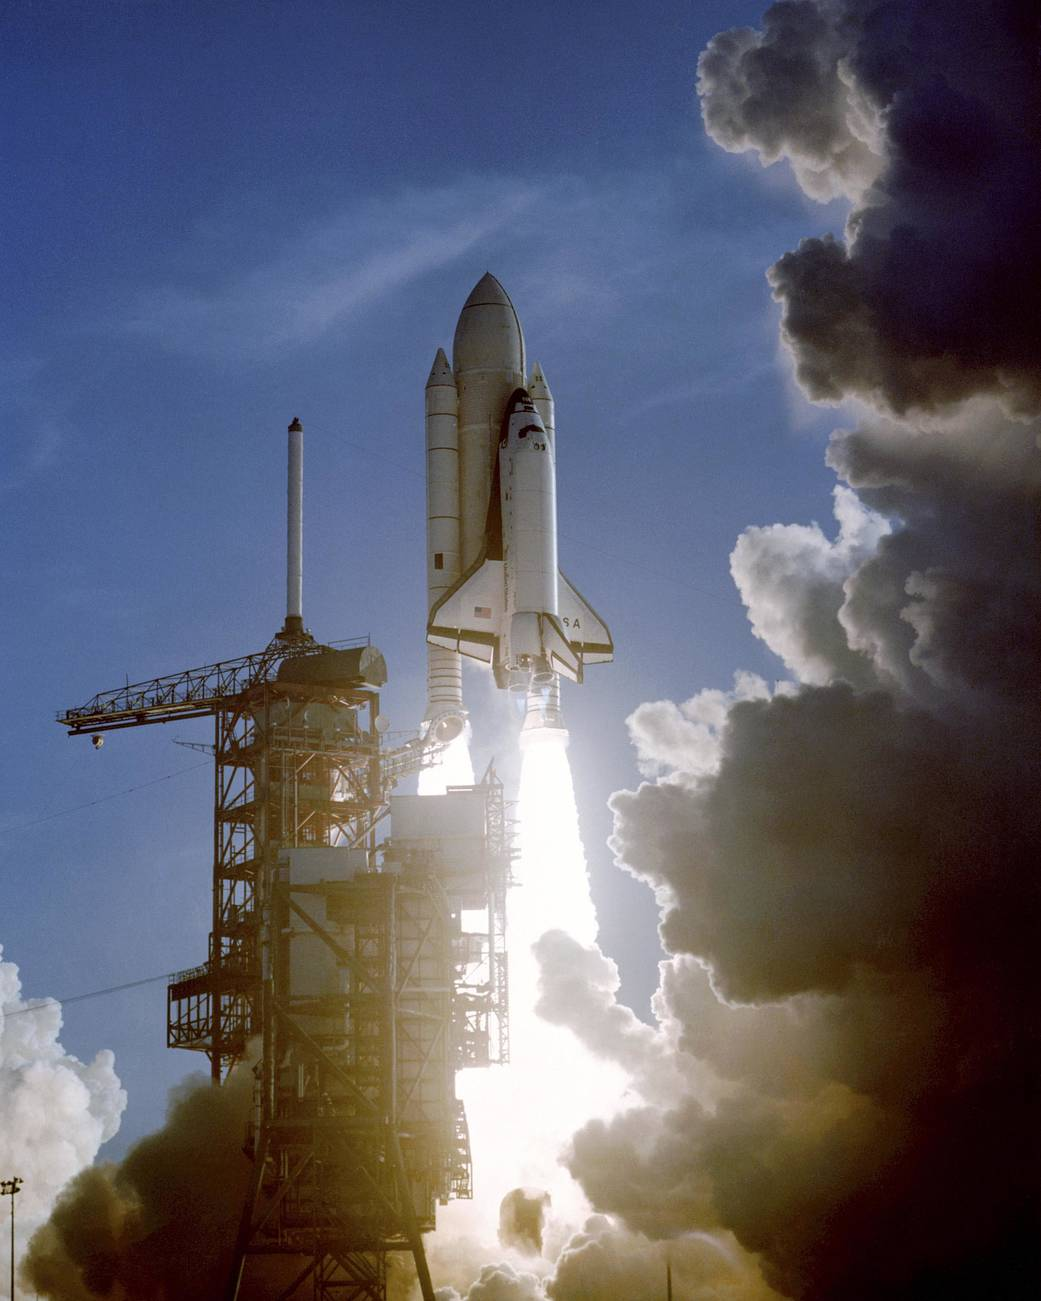
\includegraphics[height=\paperheight]{cover-nasa.jpg}};
\fill[white,opacity=.91] (0,0) rectangle (595.276,89.5);
\fill[studiumInk,opacity=.96] (0,585.5) rectangle (595.276,841.89);
\node[anchor=west,text=studiumInk,font=\sffamily\bfseries\fontsize{18}{20}\selectfont,inner sep=0pt] at (51.223,38.5){STUDIUM};
\fill[studiumCyan] (51.223,61.5) rectangle (80.8,63.7);
\node[anchor=west,text=studiumInk,font=\sffamily\fontsize{9}{11}\selectfont,inner sep=0pt] at (89.49,65.5){BIBLIOTECA DE INGENIERÍA};
\node[anchor=west,text=studiumCyan,font=\sffamily\bfseries\fontsize{10}{12}\selectfont,inner sep=0pt] at (51.223,608){MANUAL UNIVERSITARIO};
\node[anchor=north west,text=white,text width=493pt,font=\rmfamily\bfseries\fontsize{33}{36}\selectfont,inner sep=0pt] at (51.223,636){#1};
\node[anchor=west,text=white!82!studiumInk,font=\sffamily\fontsize{11}{14}\selectfont,inner sep=0pt] at (51.223,732){#2};
\node[anchor=west,text=white,font=\sffamily\bfseries\fontsize{10}{12}\selectfont,inner sep=0pt] at (51.223,758){GRADO EN INGENIERÍA AEROESPACIAL};
\node[anchor=west,text=white!82!studiumInk,font=\sffamily\fontsize{10}{12}\selectfont,inner sep=0pt] at (51.223,773){Universidad de León};
\draw[white!75!studiumInk,line width=.4pt] (51.223,786) -- (544.05,786);
\node[anchor=west,text=white!82!studiumInk,font=\sffamily\fontsize{10}{12}\selectfont,inner sep=0pt] at (51.223,810){2026};
\node[anchor=east,text=white,font=\sffamily\bfseries\fontsize{10}{12}\selectfont,inner sep=0pt] at (544.05,810){I Edición};
\end{scope}\end{tikzpicture}\null\end{titlepage}\hypersetup{pageanchor=true}}

\hypersetup{pdftitle={Tecnología Aeroespacial — Problemas resueltos originales}}
\renewcommand{\studiumvolumetype}{problemas}
\begin{document}
\studiumcover{TECNOLOGÍA\\AEROESPACIAL}{Problemas resueltos y comprobaciones}{PROBLEMAS RESUELTOS}
\frontmatter
\studiumreadingguide
\chapter*{Presentación y alcance}
Estos treinta problemas complementan los ejemplos completos del manual. Sus identificadores P01–P30 se mantienen al cambiar la paginación. Los tres simulacros tienen sus soluciones al final de este cuaderno; el documento de enunciados no contiene respuestas. Se consideran ejercicios originales de aprendizaje, sin atribuirlos al profesorado ni a convocatorias oficiales.

Las comprobaciones de cálculo, dimensiones y rutas alternativas se han ejecutado y se conservan en los informes. Una ruta alternativa puede ser un balance, una inversión o un algoritmo numérico dentro del mismo modelo: eso no demuestra por sí solo que la idealización represente una aeronave real. Las hipótesis y límites forman parte de la respuesta. Los resultados se redondean aquí a seis cifras como máximo; el código conserva precisión interna. Y designa la incógnita de cada caso, cuya magnitud queda definida por su unidad y el enunciado.
\tableofcontents
\mainmatter
\chapter*{P01 · Presión a seis kilómetros}
\addcontentsline{toc}{chapter}{P01 · Presión a seis kilómetros}
\begin{studiumworked}{P01 · Presión a seis kilómetros}
\textbf{1. Enunciado.} Calcule la presión estándar a 6000 m y explique por qué no es proporcional a la altura.

\textbf{2. Datos.}
\begin{longtable}{p{.16\linewidth}p{.35\linewidth}p{.38\linewidth}}\toprule Símbolo & Valor y unidad & Significado\\\midrule\endhead
$pb$ & $101325\,\mathrm{Pa}$ & Presión base\\
$Tb$ & $288.15\,\mathrm K$ & Temperatura base\\
$\beta$ & $0.0065\,\mathrm{K/m}$ & Descenso térmico positivo\\
$H$ & $6000\,\mathrm m$ & Altitud geopotencial\\
$g$ & $9.80665\,\mathrm{m/s^2}$ & Gravedad convencional\\
$R$ & $287.053\,\mathrm{J/(kg\,K)}$ & Constante aire\\
\bottomrule\end{longtable}
\textbf{3. Incógnita.} Se busca $Y$, expresada en $\mathrm{Pa}$.

\textbf{4. Esquema.} Una columna atmosférica une una base conocida con el nivel de cálculo.

\textbf{5. Hipótesis.} Aire seco ideal; altitud geopotencial. Equilibrio hidrostático con g0; gradiente constante en la capa.

\textbf{6. Modelo físico.} Integrar dp/p=-g dH/[R(Tb-beta H)].

\textbf{Elección y deducción del procedimiento.} Combinar $dp/dH=-\rho g$ con $\rho=p/(RT)$ y $T=T_b-\beta H$ da $dp/p=-g\,dH/[R(T_b-\beta H)]$. Integrar desde la base fija la constante y produce $\ln(p/p_b)=[g/(R\beta)]\ln(T/T_b)$.

\begin{enumerate}

\item Obtener primero la temperatura del nivel.

\[\fitmath{T=\mathrm{Tb}-\beta\cdot H}\]

\[\fitmath{T=(288.15)-(0.0065)\cdot (6000)\approx 249.15\,\mathrm{K}}\]

\item El exponente es adimensional.

\[\fitmath{a=\frac{g}{R\cdot \beta}}\]

\[\fitmath{a=\frac{(9.80665)}{(287.05287)\cdot (0.0065)}\approx 5.25588\,}\]

\item Exponenciar la relación integrada.

\[\fitmath{p=\mathrm{pb}\cdot {\left(\frac{T}{\mathrm{Tb}}\right)}^{a}}\]

\[\fitmath{p=(101325)\cdot {\left(\frac{(249.15)}{(288.15)}\right)}^{(5.255879813)}\approx 47181\,\mathrm{Pa}}\]

\end{enumerate}

\textbf{10. Resultado.} $Y=47181\,\mathrm{Pa}$.

\textbf{11. Interpretación física.} La presión disminuye; su curvatura evita extrapolar una recta hasta gran altitud.

\textbf{12. Comprobación por otra ruta.} Integre la ecuación diferencial hidrostática con un método adaptativo y compare; script check\_science.py usa una integración independiente en alturas de control. La ejecución de la ruta alternativa da $Y_{alt}=47181\,\mathrm{Pa}$, con diferencia relativa $0$. La consistencia dimensional se comprobó por separado. El alcance es el del modelo declarado.

\textbf{13. Limitaciones.} Sólo troposfera 0–11 km; no atmósfera real.

\textbf{Transferencia.} Antes de recalcular, prediga cómo cambiaría el resultado si variase un dato independiente un 5\,\%. Elija un dato que pueda cambiarse físicamente manteniendo los demás; si no puede hacerlo, explique la restricción de equilibrio o de dominio.\par
\end{studiumworked}
\chapter*{P02 · Densidad troposférica}
\addcontentsline{toc}{chapter}{P02 · Densidad troposférica}
\begin{studiumworked}{P02 · Densidad troposférica}
\textbf{1. Enunciado.} Obtenga la densidad estándar a 6000 m sin redondear primero la temperatura.

\textbf{2. Datos.}
\begin{longtable}{p{.16\linewidth}p{.35\linewidth}p{.38\linewidth}}\toprule Símbolo & Valor y unidad & Significado\\\midrule\endhead
$pb$ & $101325\,\mathrm{Pa}$ & Presión base\\
$Tb$ & $288.15\,\mathrm K$ & Temperatura base\\
$\beta$ & $0.0065\,\mathrm{K/m}$ & Descenso térmico\\
$H$ & $6000\,\mathrm m$ & Altitud\\
$g$ & $9.80665\,\mathrm{m/s^2}$ & Gravedad\\
$R$ & $287.053\,\mathrm{J/(kg\,K)}$ & Constante aire\\
\bottomrule\end{longtable}
\textbf{3. Incógnita.} Se busca $Y$, expresada en $\mathrm{kg\,m^{-3}}$.

\textbf{4. Esquema.} Una columna atmosférica une una base conocida con el nivel de cálculo.

\textbf{5. Hipótesis.} Aire seco ideal; altitud geopotencial. Equilibrio hidrostático con g0; gradiente constante en la capa.

\textbf{6. Modelo físico.} Combinar p(H) y rho=p/(RT).

\textbf{Elección y deducción del procedimiento.} La misma integración hidrostática da $p=p_b(T/T_b)^{g/(R\beta)}$. Después se usa la ecuación de estado con temperatura local, no la de la base.

\begin{enumerate}

\item Calcular la temperatura sin redondeo previo.

\[\fitmath{T=\mathrm{Tb}-\beta\cdot H}\]

\[\fitmath{T=(288.15)-(0.0065)\cdot (6000)\approx 249.15\,\mathrm{K}}\]

\item Calcular la presión de la capa.

\[\fitmath{p=\mathrm{pb}\cdot {\left(\frac{T}{\mathrm{Tb}}\right)}^{\frac{g}{R\cdot \beta}}}\]

\[\fitmath{p=(101325)\cdot {\left(\frac{(249.15)}{(288.15)}\right)}^{\frac{(9.80665)}{(287.05287)\cdot (0.0065)}}\approx 47181\,\mathrm{Pa}}\]

\item Dividir presión por constante y temperatura absoluta.

\[\fitmath{\rho=\frac{p}{R\cdot T}}\]

\[\fitmath{\rho=\frac{(47181.00219)}{(287.05287)\cdot (249.15)}\approx 0.6596968\,\mathrm{kg/m^{3}}}\]

\end{enumerate}

\textbf{10. Resultado.} $Y=0.659697\,\mathrm{kg\,m^{-3}}$.

\textbf{11. Interpretación física.} Densidad menor exige mayor TAS para igual sustentación y CL.

\textbf{12. Comprobación por otra ruta.} Compruebe rho R T=p usando P01 y T=Tb-beta H; es un cierre de estado, no evidencia independiente de la atmósfera real. La ejecución de la ruta alternativa da $Y_{alt}=0.659697\,\mathrm{kg\,m^{-3}}$, con diferencia relativa $2.22\times10^{-16}$. La consistencia dimensional se comprobó por separado. El alcance es el del modelo declarado.

\textbf{13. Limitaciones.} No incorporar humedad sin modificar la ecuación de estado.

\textbf{Transferencia.} Antes de recalcular, prediga cómo cambiaría el resultado si variase un dato independiente un 5\,\%. Elija un dato que pueda cambiarse físicamente manteniendo los demás; si no puede hacerlo, explique la restricción de equilibrio o de dominio.\par
\end{studiumworked}
\chapter*{P03 · Capa isoterma}
\addcontentsline{toc}{chapter}{P03 · Capa isoterma}
\begin{studiumworked}{P03 · Capa isoterma}
\textbf{1. Enunciado.} Determine la presión a 16 km utilizando la base de 11 km.

\textbf{2. Datos.}
\begin{longtable}{p{.16\linewidth}p{.35\linewidth}p{.38\linewidth}}\toprule Símbolo & Valor y unidad & Significado\\\midrule\endhead
$pb$ & $22632\,\mathrm{Pa}$ & Presión base\\
$Tb$ & $216.65\,\mathrm K$ & Temperatura capa\\
$dH$ & $5000\,\mathrm m$ & Salto de altitud\\
$g$ & $9.80665\,\mathrm{m/s^2}$ & Gravedad\\
$R$ & $287.053\,\mathrm{J/(kg\,K)}$ & Constante aire\\
\bottomrule\end{longtable}
\textbf{3. Incógnita.} Se busca $Y$, expresada en $\mathrm{Pa}$.

\textbf{4. Esquema.} Una columna atmosférica une una base conocida con el nivel de cálculo.

\textbf{5. Hipótesis.} Capa 11–20 km isoterma; gas ideal seco.

\textbf{6. Modelo físico.} Integración de la hidrostática con temperatura constante.

\textbf{Elección y deducción del procedimiento.} En una capa isoterma $T=T_b$, separar hidrostática da $dp/p=-g\,dH/(RT_b)$. Integrar entre la base y el nivel da $p=p_be^{-g\Delta H/(RT_b)}$.

\begin{enumerate}

\item El exponente negativo debe ser adimensional.

\[\fitmath{\mathrm{exponent}=\frac{-g\cdot \mathrm{dH}}{R\cdot \mathrm{Tb}}}\]

\[\fitmath{\mathrm{exponent}=\frac{-(9.80665)\cdot (5000)}{(287.05287)\cdot (216.65)}\approx -0.7884426\,}\]

\item Usar la presión de base de 11 km, no la del mar.

\[\fitmath{p=\mathrm{pb}\cdot \exp\left(\mathrm{exponent}\right)}\]

\[\fitmath{p=(22632.0401)\cdot \exp\left((-0.7884426213)\right)\approx 10287.44\,\mathrm{Pa}}\]

\end{enumerate}

\textbf{10. Resultado.} $Y=10287.4\,\mathrm{Pa}$.

\textbf{11. Interpretación física.} Se continúa desde la base de capa; no se reinicia con presión de nivel del mar.

\textbf{12. Comprobación por otra ruta.} El límite del modelo de gradiente cuando éste tiende a cero coincide simbólicamente con la exponencial. La ejecución de la ruta alternativa da $Y_{alt}=10287.4\,\mathrm{Pa}$, con diferencia relativa $1.77\times10^{-16}$. La consistencia dimensional se comprobó por separado. El alcance es el del modelo declarado.

\textbf{13. Limitaciones.} La altitud dada es geopotencial.

\textbf{Transferencia.} Antes de recalcular, prediga cómo cambiaría el resultado si variase un dato independiente un 5\,\%. Elija un dato que pueda cambiarse físicamente manteniendo los demás; si no puede hacerlo, explique la restricción de equilibrio o de dominio.\par
\end{studiumworked}
\chapter*{P04 · Altitud geométrica y geopotencial}
\addcontentsline{toc}{chapter}{P04 · Altitud geométrica y geopotencial}
\begin{studiumworked}{P04 · Altitud geométrica y geopotencial}
\textbf{1. Enunciado.} Convierta 14 km geométricos al argumento de la atmósfera estándar.

\textbf{2. Datos.}
\begin{longtable}{p{.16\linewidth}p{.35\linewidth}p{.38\linewidth}}\toprule Símbolo & Valor y unidad & Significado\\\midrule\endhead
$Rearth$ & $6.35677\times10^{6}\,\mathrm m$ & Radio geopotencial convencional\\
$z$ & $14000\,\mathrm m$ & Altitud geométrica\\
\bottomrule\end{longtable}
\textbf{3. Incógnita.} Se busca $Y$, expresada en $\mathrm m$.

\textbf{4. Esquema.} Una columna atmosférica une una base conocida con el nivel de cálculo.

\textbf{5. Hipótesis.} Gravedad inversa al cuadrado en el modelo esférico.

\textbf{6. Modelo físico.} Igualar potencial específico con g0 H.

\textbf{Elección y deducción del procedimiento.} Igualar $g_0H$ al incremento de potencial del campo esférico da $H=R_ez/(R_e+z)$. La altura geométrica entra tanto en numerador como denominador.

\begin{enumerate}

\item Calcular el factor menor que uno.

\[\fitmath{\mathrm{factor}=\frac{\mathrm{Rearth}}{\mathrm{Rearth}+z}}\]

\[\fitmath{\mathrm{factor}=\frac{(6356766)}{(6356766)+(14000)}\approx 0.9978025\,}\]

\item Multiplicar por altura geométrica.

\[\fitmath{H=\mathrm{factor}\cdot z}\]

\[\fitmath{H=(0.9978024621)\cdot (14000)\approx 13969.23\,\mathrm{m}}\]

\end{enumerate}

\textbf{10. Resultado.} $Y=13969.2\,\mathrm m$.

\textbf{11. Interpretación física.} H es ligeramente menor que z, no otra medida barométrica.

\textbf{12. Comprobación por otra ruta.} Sustituya H en z=Rearth H/(Rearth-H) y recupere el dato. La ejecución de la ruta alternativa da $Y_{alt}=13969.2\,\mathrm m$, con diferencia relativa $0$. La consistencia dimensional se comprobó por separado. El alcance es el del modelo declarado.

\textbf{13. Limitaciones.} No es conversión de altura elipsoidal GNSS a altitud ortométrica.

\textbf{Transferencia.} Antes de recalcular, prediga cómo cambiaría el resultado si variase un dato independiente un 5\,\%. Elija un dato que pueda cambiarse físicamente manteniendo los demás; si no puede hacerlo, explique la restricción de equilibrio o de dominio.\par
\end{studiumworked}
\chapter*{P05 · Altitud de densidad}
\addcontentsline{toc}{chapter}{P05 · Altitud de densidad}
\begin{studiumworked}{P05 · Altitud de densidad}
\textbf{1. Enunciado.} Una masa de aire tiene densidad 0.90 kg/m3. Halle su altitud de densidad troposférica.

\textbf{2. Datos.}
\begin{longtable}{p{.16\linewidth}p{.35\linewidth}p{.38\linewidth}}\toprule Símbolo & Valor y unidad & Significado\\\midrule\endhead
$\rho$ & $0.9\,\mathrm{kg\,m^{-3}}$ & Densidad observada\\
$\rho_{0}$ & $1.225\,\mathrm{kg\,m^{-3}}$ & Densidad estándar base\\
$Tb$ & $288.15\,\mathrm K$ & Temperatura base\\
$\beta$ & $0.0065\,\mathrm{K/m}$ & Descenso térmico\\
$g$ & $9.80665\,\mathrm{m/s^2}$ & Gravedad\\
$R$ & $287.053\,\mathrm{J/(kg\,K)}$ & Constante aire\\
\bottomrule\end{longtable}
\textbf{3. Incógnita.} Se busca $Y$, expresada en $\mathrm m$.

\textbf{4. Esquema.} Una columna atmosférica une una base conocida con el nivel de cálculo.

\textbf{5. Hipótesis.} Aire seco ideal; altitud geopotencial. Equilibrio hidrostático con g0; gradiente constante en la capa.

\textbf{6. Modelo físico.} Invertir la relación estándar rho(H), no integrar la atmósfera real.

\textbf{Elección y deducción del procedimiento.} En la troposfera $\rho/\rho_0=(1-\beta H/T_b)^a$ con $a=g/(R\beta)-1$. Elevar ambos lados a $1/a$, pasar términos y dividir por $\beta/T_b$ permite despejar altura.

\begin{enumerate}

\item Identificar el exponente de densidad, diferente del de presión.

\[\fitmath{a=\frac{g}{R\cdot \beta}-1}\]

\[\fitmath{a=\frac{(9.80665)}{(287.05287)\cdot (0.0065)}-1\approx 4.25588\,}\]

\item Tomar la potencia inversa del cociente de densidades.

\[\fitmath{f={\left(\frac{\rho}{rho0}\right)}^{\frac{1}{a}}}\]

\[\fitmath{f={\left(\frac{(0.9)}{(1.225000018)}\right)}^{\frac{1}{(4.255879813)}}\approx 0.9301204\,}\]

\item Aislar la altura geopotencial.

\[\fitmath{H=\frac{\mathrm{Tb}}{\beta}\cdot \left(1-f\right)}\]

\[\fitmath{H=\frac{(288.15)}{(0.0065)}\cdot \left(1-(0.9301203632)\right)\approx 3097.818\,\mathrm{m}}\]

\end{enumerate}

\textbf{10. Resultado.} $Y=3097.82\,\mathrm m$.

\textbf{11. Interpretación física.} La altitud de densidad es una equivalencia de prestaciones.

\textbf{12. Comprobación por otra ruta.} Sustituya el H hallado en rhoISA(H); la inversión debe devolver 0.90 kg/m3. La ejecución de la ruta alternativa da $Y_{alt}=3097.82\,\mathrm m$, con diferencia relativa $2.94\times10^{-16}$. La consistencia dimensional se comprobó por separado. El alcance es el del modelo declarado.

\textbf{13. Limitaciones.} La raíz debe permanecer en 0–11 km.

\textbf{Transferencia.} Antes de recalcular, prediga cómo cambiaría el resultado si variase un dato independiente un 5\,\%. Elija un dato que pueda cambiarse físicamente manteniendo los demás; si no puede hacerlo, explique la restricción de equilibrio o de dominio.\par
\end{studiumworked}
\chapter*{P06 · Mach de crucero}
\addcontentsline{toc}{chapter}{P06 · Mach de crucero}
\begin{studiumworked}{P06 · Mach de crucero}
\textbf{1. Enunciado.} Calcule Mach con TAS=175 m/s y T=249 K.

\textbf{2. Datos.}
\begin{longtable}{p{.16\linewidth}p{.35\linewidth}p{.38\linewidth}}\toprule Símbolo & Valor y unidad & Significado\\\midrule\endhead
$V$ & $175\,\mathrm{m\,s^{-1}}$ & TAS\\
$\gamma$ & $1.4\,\text{(adimensional)}$ & Razón calores\\
$R$ & $287.053\,\mathrm{J/(kg\,K)}$ & Constante aire\\
$T$ & $249\,\mathrm K$ & Temperatura estática\\
\bottomrule\end{longtable}
\textbf{3. Incógnita.} Se busca $Y$, expresada en $\text{(adimensional)}$.

\textbf{4. Esquema.} Se separan las magnitudes dadas del sistema y el resultado buscado; el modelo relaciona ambos sin introducir un dato de solución en el esquema.

\textbf{5. Hipótesis.} Gas caloríficamente perfecto.

\textbf{6. Modelo físico.} Sonido adiabático a²=gamma RT; M=V/a.

\textbf{Elección y deducción del procedimiento.} El sonido adiabático de gas ideal caloríficamente perfecto cumple $a^2=\gamma RT$. Primero obtener su raíz positiva y después dividir la velocidad verdadera por ella.

\begin{enumerate}

\item Usar temperatura estática en kelvin.

\[\fitmath{a=\sqrt{\gamma\cdot R\cdot T}}\]

\[\fitmath{a=\sqrt{(1.4)\cdot (287.05287)\cdot (249)}\approx 316.3331\,\mathrm{m/s}}\]

\item Mach es un cociente de velocidades.

\[\fitmath{M=\frac{V}{a}}\]

\[\fitmath{M=\frac{(175)}{(316.3331005)}\approx 0.5532143\,}\]

\end{enumerate}

\textbf{10. Resultado.} $Y=0.553214\,\text{(adimensional)}$.

\textbf{11. Interpretación física.} El régimen es subsónico, pero la compresibilidad no es despreciable por defecto.

\textbf{12. Comprobación por otra ruta.} Verifique V=M a; compare la presión de impacto isentrópica con q para estimar el error incompresible. La ejecución de la ruta alternativa da $Y_{alt}=0.553214\,\text{(adimensional)}$, con diferencia relativa $0$. La consistencia dimensional se comprobó por separado. El alcance es el del modelo declarado.

\textbf{13. Limitaciones.} La temperatura es estática y absoluta.

\textbf{Transferencia.} Antes de recalcular, prediga cómo cambiaría el resultado si variase un dato independiente un 5\,\%. Elija un dato que pueda cambiarse físicamente manteniendo los demás; si no puede hacerlo, explique la restricción de equilibrio o de dominio.\par
\end{studiumworked}
\chapter*{P07 · Semiángulo de Mach}
\addcontentsline{toc}{chapter}{P07 · Semiángulo de Mach}
\begin{studiumworked}{P07 · Semiángulo de Mach}
\textbf{1. Enunciado.} Una fuente se mueve a Mach 1.65. Calcule el semiángulo de su cono acústico.

\textbf{2. Datos.}
\begin{longtable}{p{.16\linewidth}p{.35\linewidth}p{.38\linewidth}}\toprule Símbolo & Valor y unidad & Significado\\\midrule\endhead
$Ma$ & $1.65\,\text{(adimensional)}$ & Número de Mach\\
\bottomrule\end{longtable}
\textbf{3. Incógnita.} Se busca $Y$, expresada en ${}^\circ$.

\textbf{4. Esquema.} Se separan las magnitudes dadas del sistema y el resultado buscado; el modelo relaciona ambos sin introducir un dato de solución en el esquema.

\textbf{5. Hipótesis.} Velocidad supersónica uniforme; medio homogéneo.

\textbf{6. Modelo físico.} Geometría de la envolvente: sin(mu)=1/M.

\textbf{Elección y deducción del procedimiento.} La geometría de la envolvente acústica da $\sin\mu=1/M$. Como el dato es supersónico, el argumento está entre cero y uno y se toma el ángulo agudo.

\begin{enumerate}

\item Comprobar el argumento del arco seno.

\[\fitmath{s=\frac{1}{\mathrm{Ma}}}\]

\[\fitmath{s=\frac{1}{(1.65)}\approx 0.6060606\,}\]

\item Convertir el ángulo de radianes a grados.

\[\fitmath{\mu=\frac{\arcsin\left(s\right)\cdot 180}{\pi}}\]

\[\fitmath{\mu=\frac{\arcsin\left((0.6060606061)\right)\cdot 180}{\pi}\approx 37.3052\,{}^{\circ}}\]

\end{enumerate}

\textbf{10. Resultado.} $Y=37.3052\,{}^\circ$.

\textbf{11. Interpretación física.} Mayor Mach estrecha el cono; el ángulo de un choque finito puede ser distinto.

\textbf{12. Comprobación por otra ruta.} Calcule seno del ángulo en radianes y recupere 1/M. La ejecución de la ruta alternativa da $Y_{alt}=37.3052\,{}^\circ$, con diferencia relativa $0$. La consistencia dimensional se comprobó por separado. El alcance es el del modelo declarado.

\textbf{13. Limitaciones.} No confundir Mach con ángulo de choque oblicuo.

\textbf{Transferencia.} Antes de recalcular, prediga cómo cambiaría el resultado si variase un dato independiente un 5\,\%. Elija un dato que pueda cambiarse físicamente manteniendo los demás; si no puede hacerlo, explique la restricción de equilibrio o de dominio.\par
\end{studiumworked}
\chapter*{P08 · Cuerda a partir de Reynolds}
\addcontentsline{toc}{chapter}{P08 · Cuerda a partir de Reynolds}
\begin{studiumworked}{P08 · Cuerda a partir de Reynolds}
\textbf{1. Enunciado.} Dimensione la cuerda del modelo de túnel a partir del Reynolds exigido.

\textbf{2. Datos.}
\begin{longtable}{p{.16\linewidth}p{.35\linewidth}p{.38\linewidth}}\toprule Símbolo & Valor y unidad & Significado\\\midrule\endhead
$Re$ & $2.7\times10^{6}\,\text{(adimensional)}$ & Reynolds\\
$\mu$ & $1.76\times10^{-5}\,\mathrm{Pa\,s}$ & Viscosidad\\
$\rho$ & $1.12\,\mathrm{kg\,m^{-3}}$ & Densidad\\
$V$ & $28\,\mathrm{m\,s^{-1}}$ & Velocidad\\
\bottomrule\end{longtable}
\textbf{3. Incógnita.} Se busca $Y$, expresada en $\mathrm m$.

\textbf{4. Esquema.} Se separan las magnitudes dadas del sistema y el resultado buscado; el modelo relaciona ambos sin introducir un dato de solución en el esquema.

\textbf{5. Hipótesis.} Flujo exterior caracterizado con cuerda y propiedades uniformes.

\textbf{6. Modelo físico.} Re=rho V c/mu.

\textbf{Elección y deducción del procedimiento.} De $\mathrm{Re}=\rho Vc/\mu$, multiplicar por viscosidad y dividir por densidad y velocidad para aislar la cuerda.

\begin{enumerate}

\item Conservar unidades SI antes de dividir.

\[\fitmath{c=\frac{\mathrm{Re}\cdot \mu}{\rho\cdot V}}\]

\[\fitmath{c=\frac{(2700000)\cdot (1.76\times10^{-5})}{(1.12)\cdot (28)}\approx 1.515306\,\mathrm{m}}\]

\end{enumerate}

\textbf{10. Resultado.} $Y=1.51531\,\mathrm m$.

\textbf{11. Interpretación física.} Una cuerda mayor permite mantener Re con menor velocidad.

\textbf{12. Comprobación por otra ruta.} Reconstruya Re con la cuerda obtenida y pruebe que duplicar V divide c por dos. La ejecución de la ruta alternativa da $Y_{alt}=1.51531\,\mathrm m$, con diferencia relativa $0$. La consistencia dimensional se comprobó por separado. El alcance es el del modelo declarado.

\textbf{13. Limitaciones.} Igualar Re no iguala Mach, rugosidad o turbulencia de entrada.

\textbf{Transferencia.} Antes de recalcular, prediga cómo cambiaría el resultado si variase un dato independiente un 5\,\%. Elija un dato que pueda cambiarse físicamente manteniendo los demás; si no puede hacerlo, explique la restricción de equilibrio o de dominio.\par
\end{studiumworked}
\chapter*{P09 · Continuidad compresible}
\addcontentsline{toc}{chapter}{P09 · Continuidad compresible}
\begin{studiumworked}{P09 · Continuidad compresible}
\textbf{1. Enunciado.} En un conducto entran aire de 1.15 kg/m3 a 130 m/s por 0.42 m2 y salen a 210 m/s por 0.31 m2. Halle rho de salida.

\textbf{2. Datos.}
\begin{longtable}{p{.16\linewidth}p{.35\linewidth}p{.38\linewidth}}\toprule Símbolo & Valor y unidad & Significado\\\midrule\endhead
$\rho_{1}$ & $1.15\,\mathrm{kg\,m^{-3}}$ & Densidad entrada\\
$A_{1}$ & $0.42\,\mathrm{m^2}$ & Área entrada\\
$V_{1}$ & $130\,\mathrm{m\,s^{-1}}$ & Velocidad entrada\\
$A_{2}$ & $0.31\,\mathrm{m^2}$ & Área salida\\
$V_{2}$ & $210\,\mathrm{m\,s^{-1}}$ & Velocidad salida\\
\bottomrule\end{longtable}
\textbf{3. Incógnita.} Se busca $Y$, expresada en $\mathrm{kg\,m^{-3}}$.

\textbf{4. Esquema.} Se separan las magnitudes dadas del sistema y el resultado buscado; el modelo relaciona ambos sin introducir un dato de solución en el esquema.

\textbf{5. Hipótesis.} Estacionario, sin fugas; valores uniformes de sección.

\textbf{6. Modelo físico.} Balance integral de masa.

\textbf{Elección y deducción del procedimiento.} El balance estacionario sin fugas conserva caudal másico: $\dot m=\rho_1A_1V_1=\rho_2A_2V_2$. Calcular el caudal entrante y despejar densidad de salida; no conservar solo $AV$.

\begin{enumerate}

\item Integrar el flujo de masa uniforme en la entrada.

\[\fitmath{\mathrm{mdot}=rho1\cdot A1\cdot V1}\]

\[\fitmath{\mathrm{mdot}=(1.15)\cdot (0.42)\cdot (130)\approx 62.79\,\mathrm{kg/s}}\]

\item Dividir por caudal volumétrico de salida.

\[\fitmath{rho2=\frac{\mathrm{mdot}}{A2\cdot V2}}\]

\[\fitmath{rho2=\frac{(62.79)}{(0.31)\cdot (210)}\approx 0.9645161\,\mathrm{kg/m^{3}}}\]

\end{enumerate}

\textbf{10. Resultado.} $Y=0.964516\,\mathrm{kg\,m^{-3}}$.

\textbf{11. Interpretación física.} La densidad cambia: A V no se conserva por sí solo.

\textbf{12. Comprobación por otra ruta.} Compare los dos caudales másicos rho A V; este cierre no fija presión ni temperatura. La ejecución de la ruta alternativa da $Y_{alt}=0.964516\,\mathrm{kg\,m^{-3}}$, con diferencia relativa $2.22\times10^{-16}$. La consistencia dimensional se comprobó por separado. El alcance es el del modelo declarado.

\textbf{13. Limitaciones.} Continuidad no determina si el conducto es adiabático o isentrópico.

\textbf{Transferencia.} Antes de recalcular, prediga cómo cambiaría el resultado si variase un dato independiente un 5\,\%. Elija un dato que pueda cambiarse físicamente manteniendo los demás; si no puede hacerlo, explique la restricción de equilibrio o de dominio.\par
\end{studiumworked}
\chapter*{P10 · Aceleración por caída de presión}
\addcontentsline{toc}{chapter}{P10 · Aceleración por caída de presión}
\begin{studiumworked}{P10 · Aceleración por caída de presión}
\textbf{1. Enunciado.} En una corriente de baja velocidad, p1-p2=420 Pa y V1=24 m/s. Halle V2 a rho=1.18 kg/m3.

\textbf{2. Datos.}
\begin{longtable}{p{.16\linewidth}p{.35\linewidth}p{.38\linewidth}}\toprule Símbolo & Valor y unidad & Significado\\\midrule\endhead
$V_{1}$ & $24\,\mathrm{m\,s^{-1}}$ & Velocidad inicial\\
$dp$ & $420\,\mathrm{Pa}$ & Caída presión\\
$\rho$ & $1.18\,\mathrm{kg\,m^{-3}}$ & Densidad\\
\bottomrule\end{longtable}
\textbf{3. Incógnita.} Se busca $Y$, expresada en $\mathrm{m\,s^{-1}}$.

\textbf{4. Esquema.} Se separan las magnitudes dadas del sistema y el resultado buscado; el modelo relaciona ambos sin introducir un dato de solución en el esquema.

\textbf{5. Hipótesis.} Estacionario, incompresible, sin viscosidad relevante en la línea seguida. Misma cota; sin máquinas ni pérdidas.

\textbf{6. Modelo físico.} Integrar Euler a lo largo de la corriente.

\textbf{Elección y deducción del procedimiento.} Bernoulli horizontal sin máquinas ni pérdidas da $\Delta p=\rho(V_2^2-V_1^2)/2$. Multiplicar por $2/\rho$ y sumar $V_1^2$ antes de tomar raíz.

\begin{enumerate}

\item Aislar el cuadrado de la velocidad final.

\[\fitmath{V2sq={V_{1}}^{2}+\frac{2\cdot \mathrm{dp}}{\rho}}\]

\[\fitmath{V2sq={(24)}^{2}+\frac{2\cdot (420)}{(1.18)}\approx 1287.864\,\mathrm{m^{2}/s^{2}}}\]

\item Escoger la raíz positiva para la celeridad.

\[\fitmath{V_{2}=\sqrt{V2sq}}\]

\[\fitmath{V_{2}=\sqrt{(1287.864407)}\approx 35.88683\,\mathrm{m/s}}\]

\end{enumerate}

\textbf{10. Resultado.} $Y=35.8868\,\mathrm{m\,s^{-1}}$.

\textbf{11. Interpretación física.} Menor presión estática acompaña mayor energía cinética específica.

\textbf{12. Comprobación por otra ruta.} Compruebe la diferencia de energías cinéticas rho(V2²−V1²)/2=dp y evalúe Mach. La ejecución de la ruta alternativa da $Y_{alt}=35.8868\,\mathrm{m\,s^{-1}}$, con diferencia relativa $0$. La consistencia dimensional se comprobó por separado. El alcance es el del modelo declarado.

\textbf{13. Limitaciones.} No trasladar la igualdad a un conducto real con pérdidas sin añadirlas.

\textbf{Transferencia.} Antes de recalcular, prediga cómo cambiaría el resultado si variase un dato independiente un 5\,\%. Elija un dato que pueda cambiarse físicamente manteniendo los demás; si no puede hacerlo, explique la restricción de equilibrio o de dominio.\par
\end{studiumworked}
\chapter*{P11 · Pitot de baja velocidad}
\addcontentsline{toc}{chapter}{P11 · Pitot de baja velocidad}
\begin{studiumworked}{P11 · Pitot de baja velocidad}
\textbf{1. Enunciado.} Un Pitot mide presión de impacto de 760 Pa en aire de densidad 1.19 kg/m3. Estime TAS y juzgue la aproximación.

\textbf{2. Datos.}
\begin{longtable}{p{.16\linewidth}p{.35\linewidth}p{.38\linewidth}}\toprule Símbolo & Valor y unidad & Significado\\\midrule\endhead
$qc$ & $760\,\mathrm{Pa}$ & Presión de impacto\\
$\rho$ & $1.19\,\mathrm{kg\,m^{-3}}$ & Densidad\\
\bottomrule\end{longtable}
\textbf{3. Incógnita.} Se busca $Y$, expresada en $\mathrm{m\,s^{-1}}$.

\textbf{4. Esquema.} Se separan las magnitudes dadas del sistema y el resultado buscado; el modelo relaciona ambos sin introducir un dato de solución en el esquema.

\textbf{5. Hipótesis.} Flujo subsónico de Mach pequeño; tomas alineadas y calibradas.

\textbf{6. Modelo físico.} pt-p=q bajo aproximación incompresible.

\textbf{Elección y deducción del procedimiento.} En el modelo Pitot incompresible ideal, $q_c=\rho V^2/2$. No se conoce por ello la temperatura: el Mach no puede obtenerse solo de estos datos.

\begin{enumerate}

\item Despejar la velocidad positiva de la diferencia de presión.

\[\fitmath{V=\sqrt{\frac{2\cdot \mathrm{qc}}{\rho}}}\]

\[\fitmath{V=\sqrt{\frac{2\cdot (760)}{(1.19)}}\approx 35.73949\,\mathrm{m/s}}\]

\end{enumerate}

\textbf{10. Resultado.} $Y=35.7395\,\mathrm{m\,s^{-1}}$.

\textbf{11. Interpretación física.} La raíz cuadrada impide que doble presión implique doble velocidad.

\textbf{12. Comprobación por otra ruta.} Calcule q del resultado y compare con una inversión compresible si se conoce p y T. La ejecución de la ruta alternativa da $Y_{alt}=35.7395\,\mathrm{m\,s^{-1}}$, con diferencia relativa $0$. La consistencia dimensional se comprobó por separado. El alcance es el del modelo declarado.

\textbf{13. Limitaciones.} No se puede verificar Mach sólo con rho y qc sin datos térmicos adicionales.

\textbf{Transferencia.} Antes de recalcular, prediga cómo cambiaría el resultado si variase un dato independiente un 5\,\%. Elija un dato que pueda cambiarse físicamente manteniendo los demás; si no puede hacerlo, explique la restricción de equilibrio o de dominio.\par
\end{studiumworked}
\chapter*{P12 · Pitot subsónico compresible}
\addcontentsline{toc}{chapter}{P12 · Pitot subsónico compresible}
\begin{studiumworked}{P12 · Pitot subsónico compresible}
\textbf{1. Enunciado.} Con p=47 kPa y pt=65 kPa, determine el Mach utilizando la relación isentrópica.

\textbf{2. Datos.}
\begin{longtable}{p{.16\linewidth}p{.35\linewidth}p{.38\linewidth}}\toprule Símbolo & Valor y unidad & Significado\\\midrule\endhead
$pt$ & $65000\,\mathrm{Pa}$ & Presión total\\
$p$ & $47000\,\mathrm{Pa}$ & Presión estática\\
$\gamma$ & $1.4\,\text{(adimensional)}$ & Razón calores\\
\bottomrule\end{longtable}
\textbf{3. Incógnita.} Se busca $Y$, expresada en $\text{(adimensional)}$.

\textbf{4. Esquema.} Se separan las magnitudes dadas del sistema y el resultado buscado; el modelo relaciona ambos sin introducir un dato de solución en el esquema.

\textbf{5. Hipótesis.} Subsónico, desaceleración isentrópica ideal hasta la toma.

\textbf{6. Modelo físico.} Relación entre presión total y estática del gas perfecto.

\textbf{Elección y deducción del procedimiento.} Partir de $p_t/p=[1+(\gamma-1)M^2/2]^{\gamma/(\gamma-1)}$. Elevar a $(\gamma-1)/\gamma$, restar uno y multiplicar por $2/(\gamma-1)$ aísla $M^2$.

\begin{enumerate}

\item Formar cociente de presiones absolutas.

\[\fitmath{\mathrm{ratio}=\frac{\mathrm{pt}}{p}}\]

\[\fitmath{\mathrm{ratio}=\frac{(65000)}{(47000)}\approx 1.382979\,}\]

\item Aplicar potencia inversa y despejar el cuadrado.

\[\fitmath{M2=\frac{2}{\mathrm{gamma}-1}\cdot \left({\mathrm{ratio}}^{\frac{\mathrm{gamma}-1}{\mathrm{gamma}}}-1\right)}\]

\[\fitmath{M2=\frac{2}{(1.4)-1}\cdot \left({(1.382978723)}^{\frac{(1.4)-1}{(1.4)}}-1\right)\approx 0.4853331\,}\]

\item Tomar la raíz positiva y comprobar rama subsónica.

\[\fitmath{M=\sqrt{M2}}\]

\[\fitmath{M=\sqrt{(0.4853330807)}\approx 0.6966585\,}\]

\end{enumerate}

\textbf{10. Resultado.} $Y=0.696659\,\text{(adimensional)}$.

\textbf{11. Interpretación física.} Se obtiene Mach sin conocer T; TAS sí exige temperatura.

\textbf{12. Comprobación por otra ruta.} Recalcule pt/p con el Mach encontrado y compruebe M<1. La ejecución de la ruta alternativa da $Y_{alt}=0.696659\,\text{(adimensional)}$, con diferencia relativa $4.44\times10^{-16}$. La consistencia dimensional se comprobó por separado. El alcance es el del modelo declarado.

\textbf{13. Limitaciones.} Supersónico exige pérdida de presión total a través del choque.

\textbf{Transferencia.} Antes de recalcular, prediga cómo cambiaría el resultado si variase un dato independiente un 5\,\%. Elija un dato que pueda cambiarse físicamente manteniendo los demás; si no puede hacerlo, explique la restricción de equilibrio o de dominio.\par
\end{studiumworked}
\chapter*{P13 · Carga útil de un globo}
\addcontentsline{toc}{chapter}{P13 · Carga útil de un globo}
\begin{studiumworked}{P13 · Carga útil de un globo}
\textbf{1. Enunciado.} Calcule la masa útil que deja un margen ascensional nulo para un globo de 380 m3, aire de 1.05 kg/m3, helio de 0.15 kg/m3 y estructura de 115 kg.

\textbf{2. Datos.}
\begin{longtable}{p{.16\linewidth}p{.35\linewidth}p{.38\linewidth}}\toprule Símbolo & Valor y unidad & Significado\\\midrule\endhead
$rhoair$ & $1.05\,\mathrm{kg\,m^{-3}}$ & Densidad aire\\
$rhogas$ & $0.15\,\mathrm{kg\,m^{-3}}$ & Densidad helio\\
$Vol$ & $380\,\mathrm{m^3}$ & Volumen\\
$ms$ & $115\,\mathrm{kg}$ & Masa estructura\\
\bottomrule\end{longtable}
\textbf{3. Incógnita.} Se busca $Y$, expresada en $\mathrm{kg}$.

\textbf{4. Esquema.} Una columna atmosférica une una base conocida con el nivel de cálculo.

\textbf{5. Hipótesis.} Volumen y densidades dados en condiciones de equilibrio. Masa del gas contabilizada por separado.

\textbf{6. Modelo físico.} Arquímedes y equilibrio de fuerzas.

\textbf{Elección y deducción del procedimiento.} Arquímedes da empuje $\rho_{aire}Vg$. En equilibrio compensa peso de gas, estructura y carga: $\rho_{aire}V=\rho_{gas}V+m_s+m_c$. Cancelar gravedad y despejar carga.

\begin{enumerate}

\item Restar masa de helio a masa de aire desplazada.

\[\fitmath{\mathrm{mnet}=\left(\mathrm{rhoair}-\mathrm{rhogas}\right)\cdot \mathrm{Vol}}\]

\[\fitmath{\mathrm{mnet}=\left((1.05)-(0.15)\right)\cdot (380)\approx 342\,\mathrm{kg}}\]

\item Restar masa estructural, sin volver a restar helio.

\[\fitmath{\mathrm{mc}=\mathrm{mnet}-\mathrm{ms}}\]

\[\fitmath{\mathrm{mc}=(342)-(115)\approx 227\,\mathrm{kg}}\]

\end{enumerate}

\textbf{10. Resultado.} $Y=227\,\mathrm{kg}$.

\textbf{11. Interpretación física.} El margen es masa transportable, no una fuerza.

\textbf{12. Comprobación por otra ruta.} Sume estructura, carga y helio y compare con la masa de aire desplazada. La ejecución de la ruta alternativa da $Y_{alt}=227\,\mathrm{kg}$, con diferencia relativa $1.25\times10^{-16}$. La consistencia dimensional se comprobó por separado. El alcance es el del modelo declarado.

\textbf{13. Limitaciones.} No incluye aceleración, venteo, expansión límite o masa de equipos omitidos.

\textbf{Transferencia.} Antes de recalcular, prediga cómo cambiaría el resultado si variase un dato independiente un 5\,\%. Elija un dato que pueda cambiarse físicamente manteniendo los demás; si no puede hacerlo, explique la restricción de equilibrio o de dominio.\par
\end{studiumworked}
\chapter*{P14 · Superficie de un ala trapezoidal}
\addcontentsline{toc}{chapter}{P14 · Superficie de un ala trapezoidal}
\begin{studiumworked}{P14 · Superficie de un ala trapezoidal}
\textbf{1. Enunciado.} Calcule la superficie alar para b=13.5 m, cr=2.4 m y ct/cr=0.48.

\textbf{2. Datos.}
\begin{longtable}{p{.16\linewidth}p{.35\linewidth}p{.38\linewidth}}\toprule Símbolo & Valor y unidad & Significado\\\midrule\endhead
$b$ & $13.5\,\mathrm m$ & Envergadura\\
$cr$ & $2.4\,\mathrm m$ & Cuerda raíz\\
$lam$ & $0.48\,\text{(adimensional)}$ & Estrechamiento\\
\bottomrule\end{longtable}
\textbf{3. Incógnita.} Se busca $Y$, expresada en $\mathrm{m^2}$.

\textbf{4. Esquema.} Se separan las magnitudes dadas del sistema y el resultado buscado; el modelo relaciona ambos sin introducir un dato de solución en el esquema.

\textbf{5. Hipótesis.} Planta trapezoidal simétrica; superficie de referencia completa.

\textbf{6. Modelo físico.} Área de dos trapecios semialares.

\textbf{Elección y deducción del procedimiento.} La cuerda varía linealmente desde $c_r$ a $c_t=\lambda c_r$ a lo largo de cada semiala. Integrar esa recta equivale a envergadura completa por cuerda media aritmética.

\begin{enumerate}

\item Calcular cuerda de punta.

\[\fitmath{\mathrm{ct}=\mathrm{lam}\cdot \mathrm{cr}}\]

\[\fitmath{\mathrm{ct}=(0.48)\cdot (2.4)\approx 1.152\,\mathrm{m}}\]

\item Sumar el área de los dos trapecios semialares.

\[\fitmath{S=\frac{b\cdot \left(\mathrm{cr}+\mathrm{ct}\right)}{2}}\]

\[\fitmath{S=\frac{(13.5)\cdot \left((2.4)+(1.152)\right)}{2}\approx 23.976\,\mathrm{m^{2}}}\]

\end{enumerate}

\textbf{10. Resultado.} $Y=23.976\,\mathrm{m^2}$.

\textbf{11. Interpretación física.} La superficie no es b multiplicado por cuerda de raíz.

\textbf{12. Comprobación por otra ruta.} Integre una cuerda que varía linealmente con la coordenada transversal; el área debe coincidir. La ejecución de la ruta alternativa da $Y_{alt}=23.976\,\mathrm{m^2}$, con diferencia relativa $1.48\times10^{-16}$. La consistencia dimensional se comprobó por separado. El alcance es el del modelo declarado.

\textbf{13. Limitaciones.} No representa superficie mojada ni planta elíptica.

\textbf{Transferencia.} Antes de recalcular, prediga cómo cambiaría el resultado si variase un dato independiente un 5\,\%. Elija un dato que pueda cambiarse físicamente manteniendo los demás; si no puede hacerlo, explique la restricción de equilibrio o de dominio.\par
\end{studiumworked}
\chapter*{P15 · Cuerda aerodinámica media}
\addcontentsline{toc}{chapter}{P15 · Cuerda aerodinámica media}
\begin{studiumworked}{P15 · Cuerda aerodinámica media}
\textbf{1. Enunciado.} Halle la CAM del ala anterior.

\textbf{2. Datos.}
\begin{longtable}{p{.16\linewidth}p{.35\linewidth}p{.38\linewidth}}\toprule Símbolo & Valor y unidad & Significado\\\midrule\endhead
$cr$ & $2.4\,\mathrm m$ & Cuerda raíz\\
$lam$ & $0.48\,\text{(adimensional)}$ & Estrechamiento\\
\bottomrule\end{longtable}
\textbf{3. Incógnita.} Se busca $Y$, expresada en $\mathrm m$.

\textbf{4. Esquema.} Se separan las magnitudes dadas del sistema y el resultado buscado; el modelo relaciona ambos sin introducir un dato de solución en el esquema.

\textbf{5. Hipótesis.} Planta trapezoidal, definición CAM=(1/S) integral c² dy.

\textbf{6. Modelo físico.} Integración geométrica de c² sobre envergadura.

\textbf{Elección y deducción del procedimiento.} La CAM se define como $\bar c=(1/S)\int_{-b/2}^{b/2}c(y)^2dy$. Para cuerda lineal, integrar el cuadrado y dividir por $S=b(c_r+c_t)/2$ da $\bar c=(2c_r/3)(1+\lambda+\lambda^2)/(1+\lambda)$.

\begin{enumerate}

\item Evaluar la combinación cuadrática de estrechamiento.

\[\fitmath{\mathrm{num}=1+\mathrm{lam}+{\mathrm{lam}}^{2}}\]

\[\fitmath{\mathrm{num}=1+(0.48)+{(0.48)}^{2}\approx 1.7104\,}\]

\item Multiplicar por la cuerda raíz y dividir por el factor de área.

\[\fitmath{\mathrm{cam}=\frac{\frac{2\cdot \mathrm{cr}}{3}\cdot \mathrm{num}}{1+\mathrm{lam}}}\]

\[\fitmath{\mathrm{cam}=\frac{\frac{2\cdot (2.4)}{3}\cdot (1.7104)}{1+(0.48)}\approx 1.849081\,\mathrm{m}}\]

\end{enumerate}

\textbf{10. Resultado.} $Y=1.84908\,\mathrm m$.

\textbf{11. Interpretación física.} La CAM difiere de S/b cuando la cuerda cambia.

\textbf{12. Comprobación por otra ruta.} En el límite lambda=1 se recupera cr; con lambda=0 se obtiene 2cr/3. La ejecución de la ruta alternativa da $Y_{alt}=1.84908\,\mathrm m$, con diferencia relativa $2.4\times10^{-16}$. La consistencia dimensional se comprobó por separado. El alcance es el del modelo declarado.

\textbf{13. Limitaciones.} La posición longitudinal de CAM exige geometría de flecha.

\textbf{Transferencia.} Antes de recalcular, prediga cómo cambiaría el resultado si variase un dato independiente un 5\,\%. Elija un dato que pueda cambiarse físicamente manteniendo los demás; si no puede hacerlo, explique la restricción de equilibrio o de dominio.\par
\end{studiumworked}
\chapter*{P16 · Pendiente del ala finita}
\addcontentsline{toc}{chapter}{P16 · Pendiente del ala finita}
\begin{studiumworked}{P16 · Pendiente del ala finita}
\textbf{1. Enunciado.} Un perfil tiene a0=5.9 rad-1. Calcule la pendiente del ala de AR=8.2 y ei=0.91.

\textbf{2. Datos.}
\begin{longtable}{p{.16\linewidth}p{.35\linewidth}p{.38\linewidth}}\toprule Símbolo & Valor y unidad & Significado\\\midrule\endhead
$a_{0}$ & $5.9\,\text{(adimensional)}$ & Pendiente perfil por radián\\
$ei$ & $0.91\,\text{(adimensional)}$ & Eficiencia envergadura\\
$AR$ & $8.2\,\text{(adimensional)}$ & Alargamiento\\
\bottomrule\end{longtable}
\textbf{3. Incógnita.} Se busca $Y$, expresada en $\text{(adimensional)}$.

\textbf{4. Esquema.} Se separan las magnitudes dadas del sistema y el resultado buscado; el modelo relaciona ambos sin introducir un dato de solución en el esquema.

\textbf{5. Hipótesis.} Teoría lineal de ala finita; sin pérdida, ala poco barrida.

\textbf{6. Modelo físico.} Incluir ángulo inducido CL/(pi ei AR).

\textbf{Elección y deducción del procedimiento.} El perfil responde al ángulo efectivo: $C_L=a_0[\alpha-\alpha_0-C_L/(\pi e_i AR)]$. Agrupar términos en $C_L$ da $C_L[1+a_0/(\pi e_i AR)]=a_0(\alpha-\alpha_0)$, de donde se lee la pendiente del ala.

\begin{enumerate}

\item La corrección por ángulo inducido aumenta el denominador.

\[\fitmath{\mathrm{factor}=1+\frac{a0}{\pi\cdot \mathrm{ei}\cdot \mathrm{AR}}}\]

\[\fitmath{\mathrm{factor}=1+\frac{(5.9)}{\pi\cdot (0.91)\cdot (8.2)}\approx 1.251679\,}\]

\item La pendiente se interpreta por radián.

\[\fitmath{a=\frac{a0}{\mathrm{factor}}}\]

\[\fitmath{a=\frac{(5.9)}{(1.25167895)}\approx 4.713669\,}\]

\end{enumerate}

\textbf{10. Resultado.} $Y=4.71367\,\text{(adimensional)}$.

\textbf{11. Interpretación física.} La pendiente tridimensional es menor que a0.

\textbf{12. Comprobación por otra ruta.} Sustituya CL=a(alpha-alpha0) en alpha efectiva; al AR infinito se recupera a0. La ejecución de la ruta alternativa da $Y_{alt}=4.71367\,\text{(adimensional)}$, con diferencia relativa $0$. La consistencia dimensional se comprobó por separado. El alcance es el del modelo declarado.

\textbf{13. Limitaciones.} La pendiente se interpreta por radián, no por grado; no corrección transónica.

\textbf{Transferencia.} Antes de recalcular, prediga cómo cambiaría el resultado si variase un dato independiente un 5\,\%. Elija un dato que pueda cambiarse físicamente manteniendo los demás; si no puede hacerlo, explique la restricción de equilibrio o de dominio.\par
\end{studiumworked}
\chapter*{P17 · Oswald con resistencia de perfil cuadrática}
\addcontentsline{toc}{chapter}{P17 · Oswald con resistencia de perfil cuadrática}
\begin{studiumworked}{P17 · Oswald con resistencia de perfil cuadrática}
\textbf{1. Enunciado.} Calcule eO si ei=0.92, AR=9 y kperfil=0.008.

\textbf{2. Datos.}
\begin{longtable}{p{.16\linewidth}p{.35\linewidth}p{.38\linewidth}}\toprule Símbolo & Valor y unidad & Significado\\\midrule\endhead
$ei$ & $0.92\,\text{(adimensional)}$ & Eficiencia envergadura\\
$AR$ & $9\,\text{(adimensional)}$ & Alargamiento\\
$kp$ & $0.008\,\text{(adimensional)}$ & Cuadrático de perfil\\
\bottomrule\end{longtable}
\textbf{3. Incógnita.} Se busca $Y$, expresada en $\text{(adimensional)}$.

\textbf{4. Esquema.} Se separan las magnitudes dadas del sistema y el resultado buscado; el modelo relaciona ambos sin introducir un dato de solución en el esquema.

\textbf{5. Hipótesis.} CD=CD0+[1/(pi ei AR)+kp] CL².

\textbf{6. Modelo físico.} Igualar coeficiente K total con 1/(pi eO AR).

\textbf{Elección y deducción del procedimiento.} Igualar el coeficiente cuadrático total $K=1/(\pi e_iAR)+k_p$ con $1/(\pi e_OAR)$. Multiplicar por $\pi AR$ y tomar el recíproco aísla $e_O$.

\begin{enumerate}

\item Sumar ambas contribuciones antes de invertir.

\[\fitmath{\mathrm{inv}=\frac{1}{\mathrm{ei}}+\pi\cdot \mathrm{AR}\cdot \mathrm{kp}}\]

\[\fitmath{\mathrm{inv}=\frac{1}{(0.92)}+\pi\cdot (9)\cdot (0.008)\approx 1.313151\,}\]

\item El resultado tiende a eficiencia inducida cuando el término de perfil se anula.

\[\fitmath{\mathrm{eO}=\frac{1}{\mathrm{inv}}}\]

\[\fitmath{\mathrm{eO}=\frac{1}{(1.313151193)}\approx 0.7615269\,}\]

\end{enumerate}

\textbf{10. Resultado.} $Y=0.761527\,\text{(adimensional)}$.

\textbf{11. Interpretación física.} eO es menor que ei en este modelo con kp positivo.

\textbf{12. Comprobación por otra ruta.} Reconstruya K por ambos métodos y pruebe el límite kp→0. La ejecución de la ruta alternativa da $Y_{alt}=0.761527\,\text{(adimensional)}$, con diferencia relativa $1.11\times10^{-16}$. La consistencia dimensional se comprobó por separado. El alcance es el del modelo declarado.

\textbf{13. Limitaciones.} eO es parámetro de ajuste, no distribución de carga pura.

\textbf{Transferencia.} Antes de recalcular, prediga cómo cambiaría el resultado si variase un dato independiente un 5\,\%. Elija un dato que pueda cambiarse físicamente manteniendo los demás; si no puede hacerlo, explique la restricción de equilibrio o de dominio.\par
\end{studiumworked}
\chapter*{P18 · Sustentación de equilibrio}
\addcontentsline{toc}{chapter}{P18 · Sustentación de equilibrio}
\begin{studiumworked}{P18 · Sustentación de equilibrio}
\textbf{1. Enunciado.} Calcule CL para W=48 kN, S=24 m2, rho=0.85 kg/m3 y TAS=85 m/s.

\textbf{2. Datos.}
\begin{longtable}{p{.16\linewidth}p{.35\linewidth}p{.38\linewidth}}\toprule Símbolo & Valor y unidad & Significado\\\midrule\endhead
$W$ & $48000\,\mathrm N$ & Peso\\
$\rho$ & $0.85\,\mathrm{kg\,m^{-3}}$ & Densidad\\
$V$ & $85\,\mathrm{m\,s^{-1}}$ & TAS\\
$S$ & $24\,\mathrm{m^2}$ & Superficie\\
\bottomrule\end{longtable}
\textbf{3. Incógnita.} Se busca $Y$, expresada en $\text{(adimensional)}$.

\textbf{4. Esquema.} Se separan las magnitudes dadas del sistema y el resultado buscado; el modelo relaciona ambos sin introducir un dato de solución en el esquema.

\textbf{5. Hipótesis.} Vuelo horizontal rectilíneo, empuje horizontal y sin aceleración.

\textbf{6. Modelo físico.} Equilibrio L=W y definición de CL de aeronave.

\textbf{Elección y deducción del procedimiento.} En vuelo horizontal uniforme, $L=W$. Usar $L=qSC_L$ y $q=\rho V^2/2$ y despejar el coeficiente.

\begin{enumerate}

\item Calcular presión dinámica de la condición.

\[\fitmath{q=\frac{\rho\cdot {V}^{2}}{2}}\]

\[\fitmath{q=\frac{(0.85)\cdot {(85)}^{2}}{2}\approx 3070.625\,\mathrm{Pa}}\]

\item Dividir peso por fuerza de referencia.

\[\fitmath{C_L=\frac{W}{q\cdot S}}\]

\[\fitmath{C_L=\frac{(48000)}{(3070.625)\cdot (24)}\approx 0.6513332\,}\]

\end{enumerate}

\textbf{10. Resultado.} $Y=0.651333\,\text{(adimensional)}$.

\textbf{11. Interpretación física.} CL aumenta al disminuir velocidad; necesita margen frente a CLmax.

\textbf{12. Comprobación por otra ruta.} Reconstruya L=qSCL y compruebe que las fuerzas verticales se equilibran. La ejecución de la ruta alternativa da $Y_{alt}=0.651333\,\text{(adimensional)}$, con diferencia relativa $0$. La consistencia dimensional se comprobó por separado. El alcance es el del modelo declarado.

\textbf{13. Limitaciones.} No introducir pendiente de perfil como si fuera del avión completo.

\textbf{Transferencia.} Antes de recalcular, prediga cómo cambiaría el resultado si variase un dato independiente un 5\,\%. Elija un dato que pueda cambiarse físicamente manteniendo los demás; si no puede hacerlo, explique la restricción de equilibrio o de dominio.\par
\end{studiumworked}
\chapter*{P19 · Empuje necesario en crucero}
\addcontentsline{toc}{chapter}{P19 · Empuje necesario en crucero}
\begin{studiumworked}{P19 · Empuje necesario en crucero}
\textbf{1. Enunciado.} Halle T necesario con los datos de P18, CD0=0.027 y K=0.049.

\textbf{2. Datos.}
\begin{longtable}{p{.16\linewidth}p{.35\linewidth}p{.38\linewidth}}\toprule Símbolo & Valor y unidad & Significado\\\midrule\endhead
$W$ & $48000\,\mathrm N$ & Peso\\
$\rho$ & $0.85\,\mathrm{kg\,m^{-3}}$ & Densidad\\
$V$ & $85\,\mathrm{m\,s^{-1}}$ & TAS\\
$S$ & $24\,\mathrm{m^2}$ & Superficie\\
$CD_{0}$ & $0.027\,\text{(adimensional)}$ & Coeficiente parásito\\
$K$ & $0.049\,\text{(adimensional)}$ & Coeficiente cuadrático\\
\bottomrule\end{longtable}
\textbf{3. Incógnita.} Se busca $Y$, expresada en $\mathrm N$.

\textbf{4. Esquema.} Se separan las magnitudes dadas del sistema y el resultado buscado; el modelo relaciona ambos sin introducir un dato de solución en el esquema.

\textbf{5. Hipótesis.} Vuelo horizontal uniforme; polar válida en el estado considerado.

\textbf{6. Modelo físico.} T=D=qSCD y CL=W/(qS).

\textbf{Elección y deducción del procedimiento.} El equilibrio tangencial exige $T=D$. Con la polar $D=qS(C_{D0}+KC_L^2)$ y $C_L=W/(qS)$, calcular sustentación, coeficiente de resistencia y fuerza en ese orden.

\begin{enumerate}

\item Formar presión dinámica.

\[\fitmath{q=\frac{\rho\cdot {V}^{2}}{2}}\]

\[\fitmath{q=\frac{(0.85)\cdot {(85)}^{2}}{2}\approx 3070.625\,\mathrm{Pa}}\]

\item Imponer equilibrio vertical.

\[\fitmath{C_L=\frac{W}{q\cdot S}}\]

\[\fitmath{C_L=\frac{(48000)}{(3070.625)\cdot (24)}\approx 0.6513332\,}\]

\item Evaluar la polar en el coeficiente requerido.

\[\fitmath{C_D=C_{D0}+K\cdot {C_L}^{2}}\]

\[\fitmath{C_D=(0.027)+(0.049)\cdot {(0.6513331976)}^{2}\approx 0.04778751\,}\]

\item Imponer equilibrio tangencial.

\[\fitmath{T=q\cdot S\cdot C_D}\]

\[\fitmath{T=(3070.625)\cdot (24)\cdot (0.04778751178)\approx 3521.701\,\mathrm{N}}\]

\end{enumerate}

\textbf{10. Resultado.} $Y=3521.7\,\mathrm N$.

\textbf{11. Interpretación física.} El motor debe proporcionar ese empuje disponible si el crucero se mantiene.

\textbf{12. Comprobación por otra ruta.} Calcule por otra ruta CL, CD y qSCD y compare con la forma A V²+B/V². La ejecución de la ruta alternativa da $Y_{alt}=3521.7\,\mathrm N$, con diferencia relativa $1.29\times10^{-16}$. La consistencia dimensional se comprobó por separado. El alcance es el del modelo declarado.

\textbf{13. Limitaciones.} No es potencia del eje ni empuje máximo del motor.

\textbf{Transferencia.} Antes de recalcular, prediga cómo cambiaría el resultado si variase un dato independiente un 5\,\%. Elija un dato que pueda cambiarse físicamente manteniendo los demás; si no puede hacerlo, explique la restricción de equilibrio o de dominio.\par
\end{studiumworked}
\chapter*{P20 · Velocidad de mínima resistencia}
\addcontentsline{toc}{chapter}{P20 · Velocidad de mínima resistencia}
\begin{studiumworked}{P20 · Velocidad de mínima resistencia}
\textbf{1. Enunciado.} Halle la TAS de mínima resistencia para el modelo de P19.

\textbf{2. Datos.}
\begin{longtable}{p{.16\linewidth}p{.35\linewidth}p{.38\linewidth}}\toprule Símbolo & Valor y unidad & Significado\\\midrule\endhead
$W$ & $48000\,\mathrm N$ & Peso\\
$\rho$ & $0.85\,\mathrm{kg\,m^{-3}}$ & Densidad\\
$S$ & $24\,\mathrm{m^2}$ & Superficie\\
$CD_{0}$ & $0.027\,\text{(adimensional)}$ & Coeficiente parásito\\
$K$ & $0.049\,\text{(adimensional)}$ & Coeficiente cuadrático\\
\bottomrule\end{longtable}
\textbf{3. Incógnita.} Se busca $Y$, expresada en $\mathrm{m\,s^{-1}}$.

\textbf{4. Esquema.} Se separan las magnitudes dadas del sistema y el resultado buscado; el modelo relaciona ambos sin introducir un dato de solución en el esquema.

\textbf{5. Hipótesis.} Modelo parabólico; parámetros constantes, vuelo nivelado.

\textbf{6. Modelo físico.} Derivar D=A V²+B/V² y anular dD/dV.

\textbf{Elección y deducción del procedimiento.} Escribir $D=AV^2+B/V^2$, con $A=\rho SC_{D0}/2$ y $B=2KW^2/(\rho S)$. Derivar da $2AV-2B/V^3=0$, luego $V^4=B/A$; la segunda derivada es positiva.

\begin{enumerate}

\item Identificar el término cuadrático de resistencia.

\[\fitmath{A=\frac{\rho\cdot S\cdot C_{D0}}{2}}\]

\[\fitmath{A=\frac{(0.85)\cdot (24)\cdot (0.027)}{2}\approx 0.2754\,\mathrm{kg/m}}\]

\item Identificar el término inversamente cuadrático.

\[\fitmath{B=\frac{2\cdot K\cdot {W}^{2}}{\rho\cdot S}}\]

\[\fitmath{B=\frac{2\cdot (0.049)\cdot {(48000)}^{2}}{(0.85)\cdot (24)}\approx 1.106824\times10^{7}\,\mathrm{N\,m^{2}/s^{2}}}\]

\item Tomar la cuarta raíz positiva.

\[\fitmath{\mathrm{Vopt}={\left(\frac{B}{A}\right)}^{0.25}}\]

\[\fitmath{\mathrm{Vopt}={\left(\frac{(11068235.29)}{(0.2754)}\right)}^{0.25}\approx 79.62118\,\mathrm{m/s}}\]

\end{enumerate}

\textbf{10. Resultado.} $Y=79.6212\,\mathrm{m\,s^{-1}}$.

\textbf{11. Interpretación física.} Equilibra resistencia parásita y término cuadrático total.

\textbf{12. Comprobación por otra ruta.} Minimice D numéricamente y contraste con la expresión cerrada. La ejecución de la ruta alternativa da $Y_{alt}=79.6212\,\mathrm{m\,s^{-1}}$, con diferencia relativa $1.07\times10^{-8}$. La consistencia dimensional se comprobó por separado. El alcance es el del modelo declarado.

\textbf{13. Limitaciones.} La velocidad óptima sólo es accesible si no viola pérdida, Mach o límites estructurales.

\textbf{Transferencia.} Antes de recalcular, prediga cómo cambiaría el resultado si variase un dato independiente un 5\,\%. Elija un dato que pueda cambiarse físicamente manteniendo los demás; si no puede hacerlo, explique la restricción de equilibrio o de dominio.\par
\end{studiumworked}
\chapter*{P21 · Velocidad de mínima potencia necesaria}
\addcontentsline{toc}{chapter}{P21 · Velocidad de mínima potencia necesaria}
\begin{studiumworked}{P21 · Velocidad de mínima potencia necesaria}
\textbf{1. Enunciado.} Calcule la TAS de mínima potencia aerodinámica para el mismo modelo.

\textbf{2. Datos.}
\begin{longtable}{p{.16\linewidth}p{.35\linewidth}p{.38\linewidth}}\toprule Símbolo & Valor y unidad & Significado\\\midrule\endhead
$W$ & $48000\,\mathrm N$ & Peso\\
$\rho$ & $0.85\,\mathrm{kg\,m^{-3}}$ & Densidad\\
$S$ & $24\,\mathrm{m^2}$ & Superficie\\
$CD_{0}$ & $0.027\,\text{(adimensional)}$ & Coeficiente parásito\\
$K$ & $0.049\,\text{(adimensional)}$ & Coeficiente cuadrático\\
\bottomrule\end{longtable}
\textbf{3. Incógnita.} Se busca $Y$, expresada en $\mathrm{m\,s^{-1}}$.

\textbf{4. Esquema.} Se separan las magnitudes dadas del sistema y el resultado buscado; el modelo relaciona ambos sin introducir un dato de solución en el esquema.

\textbf{5. Hipótesis.} Vuelo nivelado; CD0 y K constantes.

\textbf{6. Modelo físico.} Derivar Pn=A V³+B/V.

\textbf{Elección y deducción del procedimiento.} La potencia necesaria es $P=DV=AV^3+B/V$. Su derivada $3AV^2-B/V^2=0$ da $V^4=B/(3A)$. No se usa el óptimo de resistencia sin modificarlo.

\begin{enumerate}

\item Conservar el coeficiente parásito.

\[\fitmath{A=\frac{\rho\cdot S\cdot C_{D0}}{2}}\]

\[\fitmath{A=\frac{(0.85)\cdot (24)\cdot (0.027)}{2}\approx 0.2754\,\mathrm{kg/m}}\]

\item Conservar el término de sustentación.

\[\fitmath{B=\frac{2\cdot K\cdot {W}^{2}}{\rho\cdot S}}\]

\[\fitmath{B=\frac{2\cdot (0.049)\cdot {(48000)}^{2}}{(0.85)\cdot (24)}\approx 1.106824\times10^{7}\,\mathrm{N\,m^{2}/s^{2}}}\]

\item Tomar la cuarta raíz del cociente con factor tres.

\[\fitmath{\mathrm{Vopt}={\left(\frac{B}{3\cdot A}\right)}^{0.25}}\]

\[\fitmath{\mathrm{Vopt}={\left(\frac{(11068235.29)}{3\cdot (0.2754)}\right)}^{0.25}\approx 60.49901\,\mathrm{m/s}}\]

\end{enumerate}

\textbf{10. Resultado.} $Y=60.499\,\mathrm{m\,s^{-1}}$.

\textbf{11. Interpretación física.} Es menor que la velocidad de mínima resistencia por un factor $3^{-1/4}$.

\textbf{12. Comprobación por otra ruta.} Evalúe el signo de dPn/dV a ambos lados; compare su relación con P20. La ejecución de la ruta alternativa da $Y_{alt}=60.499\,\mathrm{m\,s^{-1}}$, con diferencia relativa $1.87\times10^{-9}$. La consistencia dimensional se comprobó por separado. El alcance es el del modelo declarado.

\textbf{13. Limitaciones.} Autonomía de hélice exige además modelo de consumo y rendimiento propulsivo.

\textbf{Transferencia.} Antes de recalcular, prediga cómo cambiaría el resultado si variase un dato independiente un 5\,\%. Elija un dato que pueda cambiarse físicamente manteniendo los demás; si no puede hacerlo, explique la restricción de equilibrio o de dominio.\par
\end{studiumworked}
\chapter*{P22 · Máxima eficiencia}
\addcontentsline{toc}{chapter}{P22 · Máxima eficiencia}
\begin{studiumworked}{P22 · Máxima eficiencia}
\textbf{1. Enunciado.} Calcule la eficiencia aerodinámica máxima para CD0=0.027 y K=0.049.

\textbf{2. Datos.}
\begin{longtable}{p{.16\linewidth}p{.35\linewidth}p{.38\linewidth}}\toprule Símbolo & Valor y unidad & Significado\\\midrule\endhead
$CD_{0}$ & $0.027\,\text{(adimensional)}$ & Coeficiente parásito\\
$K$ & $0.049\,\text{(adimensional)}$ & Cuadrático total\\
\bottomrule\end{longtable}
\textbf{3. Incógnita.} Se busca $Y$, expresada en $\text{(adimensional)}$.

\textbf{4. Esquema.} Se separan las magnitudes dadas del sistema y el resultado buscado; el modelo relaciona ambos sin introducir un dato de solución en el esquema.

\textbf{5. Hipótesis.} Polar parabólica; CL positivo.

\textbf{6. Modelo físico.} Derivar CL/(CD0+K CL²).

\textbf{Elección y deducción del procedimiento.} Derivar $E=C_L/(C_{D0}+KC_L^2)$ da numerador $C_{D0}-KC_L^2$. El óptimo positivo cumple $KC_L^2=C_{D0}$ y el denominador se convierte en $2C_{D0}$.

\begin{enumerate}

\item Despejar el coeficiente óptimo.

\[\fitmath{\mathrm{CLopt}=\sqrt{\frac{C_{D0}}{K}}}\]

\[\fitmath{\mathrm{CLopt}=\sqrt{\frac{(0.027)}{(0.049)}}\approx 0.7423075\,}\]

\item Evaluar la eficiencia con el óptimo.

\[\fitmath{\mathrm{Emax}=\frac{\mathrm{CLopt}}{2\cdot C_{D0}}}\]

\[\fitmath{\mathrm{Emax}=\frac{(0.742307489)}{2\cdot (0.027)}\approx 13.74643\,}\]

\end{enumerate}

\textbf{10. Resultado.} $Y=13.7464\,\text{(adimensional)}$.

\textbf{11. Interpretación física.} La eficiencia no depende directamente del peso si la polar no cambia.

\textbf{12. Comprobación por otra ruta.} Verifique que CD0=KCL² en CL=sqrt(CD0/K), y que la pendiente de L/D cambia de signo. La ejecución de la ruta alternativa da $Y_{alt}=13.7464\,\text{(adimensional)}$, con diferencia relativa $1.5\times10^{-13}$. La consistencia dimensional se comprobó por separado. El alcance es el del modelo declarado.

\textbf{13. Limitaciones.} No implica igualdad de resistencia inducida aislada y parásita con kp no nulo.

\textbf{Transferencia.} Antes de recalcular, prediga cómo cambiaría el resultado si variase un dato independiente un 5\,\%. Elija un dato que pueda cambiarse físicamente manteniendo los demás; si no puede hacerlo, explique la restricción de equilibrio o de dominio.\par
\end{studiumworked}
\chapter*{P23 · Ascenso estacionario}
\addcontentsline{toc}{chapter}{P23 · Ascenso estacionario}
\begin{studiumworked}{P23 · Ascenso estacionario}
\textbf{1. Enunciado.} Una aeronave de 42 kN vuela a 72 m/s, con T=5.2 kN y D=3.0 kN. Halle régimen de ascenso.

\textbf{2. Datos.}
\begin{longtable}{p{.16\linewidth}p{.35\linewidth}p{.38\linewidth}}\toprule Símbolo & Valor y unidad & Significado\\\midrule\endhead
$T$ & $5200\,\mathrm N$ & Empuje disponible\\
$D$ & $3000\,\mathrm N$ & Resistencia en el estado\\
$V$ & $72\,\mathrm{m\,s^{-1}}$ & TAS\\
$W$ & $42000\,\mathrm N$ & Peso\\
\bottomrule\end{longtable}
\textbf{3. Incógnita.} Se busca $Y$, expresada en $\mathrm{m\,s^{-1}}$.

\textbf{4. Esquema.} Se separan las magnitudes dadas del sistema y el resultado buscado; el modelo relaciona ambos sin introducir un dato de solución en el esquema.

\textbf{5. Hipótesis.} Ascenso rectilíneo uniforme, empuje alineado con trayectoria. D es la resistencia del estado de ascenso, no una imposición de L=W.

\textbf{6. Modelo físico.} Balance tangencial T-D=W sin(gamma); ROC=V sin(gamma).

\textbf{Elección y deducción del procedimiento.} En ascenso rectilíneo uniforme, $T-D=W\sin\gamma$. La componente vertical de velocidad es $V\sin\gamma$. Sustituir el equilibrio produce $ROC=(T-D)V/W$.

\begin{enumerate}

\item Comprobar que el seno sea físicamente posible.

\[\fitmath{s=\frac{T-D}{W}}\]

\[\fitmath{s=\frac{(5200)-(3000)}{(42000)}\approx 0.05238095\,}\]

\item La potencia excedente se convierte en ganancia de altura.

\[\fitmath{\mathrm{ROC}=V\cdot s}\]

\[\fitmath{\mathrm{ROC}=(72)\cdot (0.05238095238)\approx 3.771429\,\mathrm{m/s}}\]

\end{enumerate}

\textbf{10. Resultado.} $Y=3.77143\,\mathrm{m\,s^{-1}}$.

\textbf{11. Interpretación física.} La potencia excedente se transforma en energía potencial por unidad de tiempo.

\textbf{12. Comprobación por otra ruta.} Compruebe W ROC=(T-D)V y que |T-D|/W<=1. La ejecución de la ruta alternativa da $Y_{alt}=3.77143\,\mathrm{m\,s^{-1}}$, con diferencia relativa $0$. La consistencia dimensional se comprobó por separado. El alcance es el del modelo declarado.

\textbf{13. Limitaciones.} Si cambia velocidad, parte de potencia modifica energía cinética.

\textbf{Transferencia.} Antes de recalcular, prediga cómo cambiaría el resultado si variase un dato independiente un 5\,\%. Elija un dato que pueda cambiarse físicamente manteniendo los demás; si no puede hacerlo, explique la restricción de equilibrio o de dominio.\par
\end{studiumworked}
\chapter*{P24 · Planeo sin viento}
\addcontentsline{toc}{chapter}{P24 · Planeo sin viento}
\begin{studiumworked}{P24 · Planeo sin viento}
\textbf{1. Enunciado.} Desde 2100 m sobre el destino, estime alcance horizontal con L/D=15.5.

\textbf{2. Datos.}
\begin{longtable}{p{.16\linewidth}p{.35\linewidth}p{.38\linewidth}}\toprule Símbolo & Valor y unidad & Significado\\\midrule\endhead
$height$ & $2100\,\mathrm m$ & Altura disponible\\
$LD$ & $15.5\,\text{(adimensional)}$ & Eficiencia\\
\bottomrule\end{longtable}
\textbf{3. Incógnita.} Se busca $Y$, expresada en $\mathrm m$.

\textbf{4. Esquema.} Se separan las magnitudes dadas del sistema y el resultado buscado; el modelo relaciona ambos sin introducir un dato de solución en el esquema.

\textbf{5. Hipótesis.} Planeo estabilizado en aire quieto; eficiencia constante; terreno plano.

\textbf{6. Modelo físico.} tan(gamma\_desc)=D/L; distancia horizontal=h L/D.

\textbf{Elección y deducción del procedimiento.} En planeo estabilizado, $\tan|\gamma|=D/L$. En el triángulo de la trayectoria, altura/alcance horizontal tiene ese mismo cociente. Despejar alcance da $R=hL/D$.

\begin{enumerate}

\item Multiplicar la altura disponible por la eficiencia impuesta.

\[\fitmath{R=\mathrm{height}\cdot \mathrm{LD}}\]

\[\fitmath{R=(2100)\cdot (15.5)\approx 32550\,\mathrm{m}}\]

\end{enumerate}

\textbf{10. Resultado.} $Y=32550\,\mathrm m$.

\textbf{11. Interpretación física.} El resultado es geométrico ideal, sin reserva ni maniobra de aproximación.

\textbf{12. Comprobación por otra ruta.} Dibuje triángulo trayectoria y recupere altura a partir de tan(gamma). La ejecución de la ruta alternativa da $Y_{alt}=32550\,\mathrm m$, con diferencia relativa $0$. La consistencia dimensional se comprobó por separado. El alcance es el del modelo declarado.

\textbf{13. Limitaciones.} Viento, virajes, hélice en molinete y configuración alteran el alcance.

\textbf{Transferencia.} Antes de recalcular, prediga cómo cambiaría el resultado si variase un dato independiente un 5\,\%. Elija un dato que pueda cambiarse físicamente manteniendo los demás; si no puede hacerlo, explique la restricción de equilibrio o de dominio.\par
\end{studiumworked}
\chapter*{P25 · Radio de giro coordinado}
\addcontentsline{toc}{chapter}{P25 · Radio de giro coordinado}
\begin{studiumworked}{P25 · Radio de giro coordinado}
\textbf{1. Enunciado.} Halle el radio de giro horizontal coordinado a 80 m/s e inclinación 30 grados.

\textbf{2. Datos.}
\begin{longtable}{p{.16\linewidth}p{.35\linewidth}p{.38\linewidth}}\toprule Símbolo & Valor y unidad & Significado\\\midrule\endhead
$V$ & $80\,\mathrm{m\,s^{-1}}$ & TAS\\
$\phi$ & $0.523599\,\text{(adimensional)}$ & Inclinación en radianes\\
$g$ & $9.80665\,\mathrm{m/s^2}$ & Gravedad\\
\bottomrule\end{longtable}
\textbf{3. Incógnita.} Se busca $Y$, expresada en $\mathrm m$.

\textbf{4. Esquema.} Se separan las magnitudes dadas del sistema y el resultado buscado; el modelo relaciona ambos sin introducir un dato de solución en el esquema.

\textbf{5. Hipótesis.} Giro horizontal estacionario, sin resbalamiento; viento no altera radio relativo al aire.

\textbf{6. Modelo físico.} Lcos(phi)=W; Lsin(phi)=mV²/r.

\textbf{Elección y deducción del procedimiento.} En viraje horizontal coordinado, $L\cos\phi=W$ y $L\sin\phi=mV^2/r$. Dividir ambas elimina $L$ y da $\tan\phi=V^2/(rg)$, que se despeja para el radio.

\begin{enumerate}

\item Obtener aceleración centrípeta de la inclinación.

\[\fitmath{\mathrm{acc}=g\cdot \tan\left(\varphi\right)}\]

\[\fitmath{\mathrm{acc}=(9.80665)\cdot \tan\left((0.5235987756)\right)\approx 5.661872\,\mathrm{m/s^{2}}}\]

\item Dividir velocidad al cuadrado por aceleración.

\[\fitmath{r=\frac{{V}^{2}}{\mathrm{acc}}}\]

\[\fitmath{r=\frac{{(80)}^{2}}{(5.661872017)}\approx 1130.368\,\mathrm{m}}\]

\end{enumerate}

\textbf{10. Resultado.} $Y=1130.37\,\mathrm m$.

\textbf{11. Interpretación física.} La inclinación aumenta carga y velocidad de pérdida.

\textbf{12. Comprobación por otra ruta.} Compruebe aceleración V²/r=g tan(phi) y n=1/cos(phi). La ejecución de la ruta alternativa da $Y_{alt}=1130.37\,\mathrm m$, con diferencia relativa $0$. La consistencia dimensional se comprobó por separado. El alcance es el del modelo declarado.

\textbf{13. Limitaciones.} Trayectoria sobre suelo con viento puede no ser circular.

\textbf{Transferencia.} Antes de recalcular, prediga cómo cambiaría el resultado si variase un dato independiente un 5\,\%. Elija un dato que pueda cambiarse físicamente manteniendo los demás; si no puede hacerlo, explique la restricción de equilibrio o de dominio.\par
\end{studiumworked}
\chapter*{P26 · Margen estático}
\addcontentsline{toc}{chapter}{P26 · Margen estático}
\begin{studiumworked}{P26 · Margen estático}
\textbf{1. Enunciado.} Con punto neutro en 0.41 CAM y CG en 0.29 CAM, determine margen estático.

\textbf{2. Datos.}
\begin{longtable}{p{.16\linewidth}p{.35\linewidth}p{.38\linewidth}}\toprule Símbolo & Valor y unidad & Significado\\\midrule\endhead
$hn$ & $0.41\,\text{(adimensional)}$ & Punto neutro relativo a CAM\\
$hcg$ & $0.29\,\text{(adimensional)}$ & CG relativo a CAM\\
\bottomrule\end{longtable}
\textbf{3. Incógnita.} Se busca $Y$, expresada en $\text{(adimensional)}$.

\textbf{4. Esquema.} Se separan las magnitudes dadas del sistema y el resultado buscado; el modelo relaciona ambos sin introducir un dato de solución en el esquema.

\textbf{5. Hipótesis.} Configuración fija, mandos bloqueados; modelo longitudinal lineal.

\textbf{6. Modelo físico.} SM=(xNP-xCG)/CAM.

\textbf{Elección y deducción del procedimiento.} Las posiciones se expresan desde el mismo origen y en unidades de CAM. El margen estático es la distancia del CG al punto neutro, positiva si este queda detrás.

\begin{enumerate}

\item Restar posiciones conservando el orden y el signo.

\[\fitmath{\mathrm{SM}=\mathrm{hn}-\mathrm{hcg}}\]

\[\fitmath{\mathrm{SM}=(0.41)-(0.29)\approx 0.12\,}\]

\end{enumerate}

\textbf{10. Resultado.} $Y=0.12\,\text{(adimensional)}$.

\textbf{11. Interpretación física.} Margen positivo favorece estabilidad estática longitudinal.

\textbf{12. Comprobación por otra ruta.} Con CLa positivo, Cmα=-CLa SM es negativo. La ejecución de la ruta alternativa da $Y_{alt}=0.12\,\text{(adimensional)}$, con diferencia relativa $0$. La consistencia dimensional se comprobó por separado. El alcance es el del modelo declarado.

\textbf{13. Limitaciones.} No establece amortiguamiento dinámico ni autoridad suficiente del timón.

\textbf{Transferencia.} Antes de recalcular, prediga cómo cambiaría el resultado si variase un dato independiente un 5\,\%. Elija un dato que pueda cambiarse físicamente manteniendo los demás; si no puede hacerlo, explique la restricción de equilibrio o de dominio.\par
\end{studiumworked}
\chapter*{P27 · Corrección de viento cruzado}
\addcontentsline{toc}{chapter}{P27 · Corrección de viento cruzado}
\begin{studiumworked}{P27 · Corrección de viento cruzado}
\textbf{1. Enunciado.} Con TAS 70 m/s y viento transversal de 12 m/s, halle la corrección angular para mantener derrota.

\textbf{2. Datos.}
\begin{longtable}{p{.16\linewidth}p{.35\linewidth}p{.38\linewidth}}\toprule Símbolo & Valor y unidad & Significado\\\midrule\endhead
$cross$ & $12\,\mathrm{m\,s^{-1}}$ & Viento transversal\\
$V$ & $70\,\mathrm{m\,s^{-1}}$ & TAS\\
\bottomrule\end{longtable}
\textbf{3. Incógnita.} Se busca $Y$, expresada en ${}^\circ$.

\textbf{4. Esquema.} Se separan las magnitudes dadas del sistema y el resultado buscado; el modelo relaciona ambos sin introducir un dato de solución en el esquema.

\textbf{5. Hipótesis.} Viento estacionario, horizontal; deriva compensada exactamente.

\textbf{6. Modelo físico.} Anular componente transversal de Va+Vw.

\textbf{Elección y deducción del procedimiento.} Para mantener derrota, la componente transversal de velocidad aérea debe cancelar al viento: $V\sin\chi_c=|V_{w,\perp}|$. Se despeja el ángulo agudo y el morro apunta hacia el lado de procedencia del viento.

\begin{enumerate}

\item Comprobar que el viento transversal no exceda la TAS.

\[\fitmath{s=\frac{\mathrm{cross}}{V}}\]

\[\fitmath{s=\frac{(12)}{(70)}\approx 0.1714286\,}\]

\item Aplicar arco seno y convertir a grados.

\[\fitmath{\mathrm{angle}=\frac{\arcsin\left(s\right)\cdot 180}{\pi}}\]

\[\fitmath{\mathrm{angle}=\frac{\arcsin\left((0.1714285714)\right)\cdot 180}{\pi}\approx 9.87089\,{}^{\circ}}\]

\end{enumerate}

\textbf{10. Resultado.} $Y=9.87089\,{}^\circ$.

\textbf{11. Interpretación física.} El morro debe orientarse hacia el viento, con signo según el lado de procedencia.

\textbf{12. Comprobación por otra ruta.} Proyecte V sin(corrección) y recupere 12 m/s. La ejecución de la ruta alternativa da $Y_{alt}=9.87089\,{}^\circ$, con diferencia relativa $0$. La consistencia dimensional se comprobó por separado. El alcance es el del modelo declarado.

\textbf{13. Limitaciones.} Requiere |cross|<=V; sin viento longitudinal todavía no se conoce velocidad sobre suelo completa.

\textbf{Transferencia.} Antes de recalcular, prediga cómo cambiaría el resultado si variase un dato independiente un 5\,\%. Elija un dato que pueda cambiarse físicamente manteniendo los demás; si no puede hacerlo, explique la restricción de equilibrio o de dominio.\par
\end{studiumworked}
\chapter*{P28 · Velocidad orbital circular}
\addcontentsline{toc}{chapter}{P28 · Velocidad orbital circular}
\begin{studiumworked}{P28 · Velocidad orbital circular}
\textbf{1. Enunciado.} Calcule velocidad circular terrestre a radio 6971 km.

\textbf{2. Datos.}
\begin{longtable}{p{.16\linewidth}p{.35\linewidth}p{.38\linewidth}}\toprule Símbolo & Valor y unidad & Significado\\\midrule\endhead
$\mu$ & $3.986\times10^{14}\,\mathrm{m^3/s^2}$ & Parámetro gravitatorio educativo\\
$r$ & $6.971\times10^{6}\,\mathrm m$ & Radio desde centro\\
\bottomrule\end{longtable}
\textbf{3. Incógnita.} Se busca $Y$, expresada en $\mathrm{m\,s^{-1}}$.

\textbf{4. Esquema.} Se separan las magnitudes dadas del sistema y el resultado buscado; el modelo relaciona ambos sin introducir un dato de solución en el esquema.

\textbf{5. Hipótesis.} Dos cuerpos; órbita circular; no atmósfera ni oblaticidad.

\textbf{6. Modelo físico.} Aceleración gravitatoria igual a centrípeta.

\textbf{Elección y deducción del procedimiento.} En órbita circular de dos cuerpos, la aceleración gravitatoria $\mu/r^2$ iguala la centrípeta $V^2/r$. Multiplicar por $r$ y tomar raíz positiva da $V=\sqrt{\mu/r}$.

\begin{enumerate}

\item Usar radio al centro, no altitud sobre la superficie.

\[\fitmath{V=\sqrt{\frac{\mu}{r}}}\]

\[\fitmath{V=\sqrt{\frac{(3.986004418\times10^{14})}{(6971000)}}\approx 7561.733\,\mathrm{m/s}}\]

\end{enumerate}

\textbf{10. Resultado.} $Y=7561.73\,\mathrm{m\,s^{-1}}$.

\textbf{11. Interpretación física.} La velocidad depende del radio al centro, no sólo de la altura.

\textbf{12. Comprobación por otra ruta.} Verifique energía específica -mu/(2r) y periodo 2pi r/V. La ejecución de la ruta alternativa da $Y_{alt}=7561.73\,\mathrm{m\,s^{-1}}$, con diferencia relativa $0$. La consistencia dimensional se comprobó por separado. El alcance es el del modelo declarado.

\textbf{13. Limitaciones.} No confundir velocidad orbital con velocidad de escape.

\textbf{Transferencia.} Antes de recalcular, prediga cómo cambiaría el resultado si variase un dato independiente un 5\,\%. Elija un dato que pueda cambiarse físicamente manteniendo los demás; si no puede hacerlo, explique la restricción de equilibrio o de dominio.\par
\end{studiumworked}
\chapter*{P29 · Delta v ideal de una etapa}
\addcontentsline{toc}{chapter}{P29 · Delta v ideal de una etapa}
\begin{studiumworked}{P29 · Delta v ideal de una etapa}
\textbf{1. Enunciado.} Calcule el incremento ideal de velocidad con Isp=305 s y relación de masas 3.2.

\textbf{2. Datos.}
\begin{longtable}{p{.16\linewidth}p{.35\linewidth}p{.38\linewidth}}\toprule Símbolo & Valor y unidad & Significado\\\midrule\endhead
$Isp$ & $305\,\mathrm s$ & Impulso específico\\
$g$ & $9.80665\,\mathrm{m/s^2}$ & Gravedad convencional\\
$ratio$ & $3.2\,\text{(adimensional)}$ & Masa inicial/final\\
\bottomrule\end{longtable}
\textbf{3. Incógnita.} Se busca $Y$, expresada en $\mathrm{m\,s^{-1}}$.

\textbf{4. Esquema.} Se separan las magnitudes dadas del sistema y el resultado buscado; el modelo relaciona ambos sin introducir un dato de solución en el esquema.

\textbf{5. Hipótesis.} Isp constante; etapa aislada; sin gravedad, resistencia o maniobras.

\textbf{6. Modelo físico.} Conservación del momento e integración de dm/m.

\textbf{Elección y deducción del procedimiento.} La conservación de momento de una etapa ideal da $dv=-c\,dm/m$, con $c=I_{sp}g_0$. Integrar entre masas inicial y final da $\Delta v=c\ln(m_i/m_f)$.

\begin{enumerate}

\item Convertir impulso específico a velocidad efectiva.

\[\fitmath{c=\mathrm{Isp}\cdot g}\]

\[\fitmath{c=(305)\cdot (9.80665)\approx 2991.028\,\mathrm{m/s}}\]

\item Usar logaritmo natural de la razón de masas.

\[\fitmath{\mathrm{dv}=c\cdot \ln\left(\mathrm{ratio}\right)}\]

\[\fitmath{\mathrm{dv}=(2991.02825)\cdot \ln\left((3.2)\right)\approx 3479.017\,\mathrm{m/s}}\]

\end{enumerate}

\textbf{10. Resultado.} $Y=3479.02\,\mathrm{m\,s^{-1}}$.

\textbf{11. Interpretación física.} La relación de masas entra logarítmicamente; la masa final incluye estructura y carga.

\textbf{12. Comprobación por otra ruta.} Integre -c dm/m numéricamente y compare con el logaritmo. La ejecución de la ruta alternativa da $Y_{alt}=3479.02\,\mathrm{m\,s^{-1}}$, con diferencia relativa $0$. La consistencia dimensional se comprobó por separado. El alcance es el del modelo declarado.

\textbf{13. Limitaciones.} No es velocidad orbital alcanzada desde la superficie con pérdidas.

\textbf{Transferencia.} Antes de recalcular, prediga cómo cambiaría el resultado si variase un dato independiente un 5\,\%. Elija un dato que pueda cambiarse físicamente manteniendo los demás; si no puede hacerlo, explique la restricción de equilibrio o de dominio.\par
\end{studiumworked}
\chapter*{P30 · Potencia hidráulica}
\addcontentsline{toc}{chapter}{P30 · Potencia hidráulica}
\begin{studiumworked}{P30 · Potencia hidráulica}
\textbf{1. Enunciado.} Una bomba entrega 0.00075 m3/s con salto de 18 MPa y rendimiento 0.84. Halle potencia de entrada.

\textbf{2. Datos.}
\begin{longtable}{p{.16\linewidth}p{.35\linewidth}p{.38\linewidth}}\toprule Símbolo & Valor y unidad & Significado\\\midrule\endhead
$dp$ & $1.8\times10^{7}\,\mathrm{Pa}$ & Incremento presión\\
$Q$ & $0.00075\,\mathrm{m^3/s}$ & Caudal\\
$\eta$ & $0.84\,\text{(adimensional)}$ & Rendimiento\\
\bottomrule\end{longtable}
\textbf{3. Incógnita.} Se busca $Y$, expresada en $\mathrm W$.

\textbf{4. Esquema.} Se separan las magnitudes dadas del sistema y el resultado buscado; el modelo relaciona ambos sin introducir un dato de solución en el esquema.

\textbf{5. Hipótesis.} Régimen estacionario; rendimiento global dado, 0<eta<=1.

\textbf{6. Modelo físico.} Potencia útil dp Q y definición eta=Pu/Pentrada.

\textbf{Elección y deducción del procedimiento.} La potencia hidráulica útil es trabajo por volumen $\Delta p$ por caudal $Q$. El rendimiento se define como $\eta=P_u/P_{entrada}$; despejar entrada implica dividir, no multiplicar, por el rendimiento.

\begin{enumerate}

\item Calcular potencia útil transferida al líquido.

\[\fitmath{\mathrm{Pu}=\mathrm{dp}\cdot Q}\]

\[\fitmath{\mathrm{Pu}=(18000000)\cdot (0.00075)\approx 13500\,\mathrm{W}}\]

\item Obtener la demanda de entrada, mayor que la útil.

\[\fitmath{\mathrm{Pin}=\frac{\mathrm{Pu}}{\eta}}\]

\[\fitmath{\mathrm{Pin}=\frac{(13500)}{(0.84)}\approx 16071.43\,\mathrm{W}}\]

\end{enumerate}

\textbf{10. Resultado.} $Y=16071.4\,\mathrm W$.

\textbf{11. Interpretación física.} Las pérdidas elevan la demanda sobre dpQ.

\textbf{12. Comprobación por otra ruta.} Calcule pérdida Pentrada-dpQ y compruebe que es positiva. La ejecución de la ruta alternativa da $Y_{alt}=16071.4\,\mathrm W$, con diferencia relativa $1.13\times10^{-16}$. La consistencia dimensional se comprobó por separado. El alcance es el del modelo declarado.

\textbf{13. Limitaciones.} No predice calentamiento sin balance térmico ni caudal de fugas.

\textbf{Transferencia.} Antes de recalcular, prediga cómo cambiaría el resultado si variase un dato independiente un 5\,\%. Elija un dato que pueda cambiarse físicamente manteniendo los demás; si no puede hacerlo, explique la restricción de equilibrio o de dominio.\par
\end{studiumworked}
\chapter{Soluciones y criterios de los simulacros}
Cada apartado se evalúa por modelo, hipótesis, desarrollo y resultado. Un resultado correcto sin justificación no demuestra la competencia completa. Las tolerancias deben reflejar las constantes y redondeos adoptados; las cifras siguientes conservan más precisión de la necesaria para presentar el examen.
\section{Simulacro 1}
Altitud de presión invierte $p_{ISA}(H)$; altitud de densidad invierte $\rho_{ISA}(H)$. A presión fija, aumentar $T$ disminuye $\rho$ y eleva la altitud de densidad. $q=\rho V^2/2$ es una escala cinética y $q_c=p_t-p$ una medida de presión; coinciden aproximadamente en Mach pequeño bajo las hipótesis de Bernoulli. Línea de corriente es tangente al campo instantáneo; trayectoria sigue una partícula. En flujo estacionario sus curvas coinciden si el campo es regular.

Para el globo se usa ISA troposférica, gas ideal para el helio y Arquímedes. Los resultados son:
\[T=265.4\,\mathrm K,\quad p=65764.1\,\mathrm{Pa},\quad \rho_a=0.863229\,\mathrm{kg/m^3}.\]
La densidad del helio es $\rho_h=p/(R_hT)=0.119297\,\mathrm{kg/m^3}$. El balance $(\rho_a-\rho_h)Vg_0=(m_s+m_u)g_0$ proporciona $m_u=234.769\,\mathrm{kg}$. Con cinco kilogramos menos queda una fuerza neta ascendente $5g_0=49.0333\,\mathrm N$. Sin un modelo de resistencia y geometría no se calcula una velocidad terminal. Una comprobación de masa consiste en sumar carga, estructura y helio: coincide con la masa de aire desplazada en equilibrio.

En el Pitot, $p=50506.8\,\mathrm{Pa}$, $T=252.4\,\mathrm K$ y $\rho=0.697105\,\mathrm{kg/m^3}$. La inversión isentrópica da $M=0.301755$ y $V=M\sqrt{\gamma RT}=96.1047\,\mathrm{m/s}$. Bernoulli incompresible produce $97.2022\,\mathrm{m/s}$, con error relativo $1.14207\,\%$. Se comprueba el Mach subsónico y se reconstruye $p_t/p$ desde el resultado. La comparación cuantifica una aproximación de modelo; no calibra un instrumento real.

En continuidad, $\dot m=\rho_1A_1V_1=46.0\,\mathrm{kg/s}$ y $V_2=\dot m/(\rho_2A_2)=125.17\,\mathrm{m/s}$. No se conserva $AV$ porque cambia $\rho$. La presión de salida requiere una relación termodinámica y balances adicionales con condiciones de contorno; continuidad sola no la determina. Se verifica el mismo caudal másico en ambas secciones.

\subsection*{Procedimiento y operaciones del simulacro 1}
Primero se obtiene el estado ISA con la altitud geopotencial. Después, la ley del gas permite calcular ambas densidades y Arquímedes cierra el equilibrio. En el Pitot se despeja Mach de la relación isentrópica antes de calcular TAS; continuidad constituye un balance separado.

\begin{enumerate}

\item Integrar el gradiente troposférico.

\[\fitmath{\mathrm{Tg}=288.15-0.0065\cdot 3500\approx 265.4\,\mathrm{K}}\]

\item Integrar equilibrio hidrostático y gas perfecto.

\[\fitmath{\mathrm{pg}=101325\cdot {\left(\frac{\mathrm{Tg}}{288.15}\right)}^{\frac{9.80665}{287.05287\cdot 0.0065}}}\]

\[\fitmath{\mathrm{pg}=101325\cdot {\left(\frac{(265.4)}{288.15}\right)}^{\frac{9.80665}{287.05287\cdot 0.0065}}\approx 65764.06\,\mathrm{Pa}}\]

\item Densidad del aire.

\[\fitmath{\mathrm{rg}=\frac{\mathrm{pg}}{287.05287\cdot \mathrm{Tg}}}\]

\[\fitmath{\mathrm{rg}=\frac{(65764.06436)}{287.05287\cdot (265.4)}\approx 0.8632286\,\mathrm{kg/m^{3}}}\]

\item Densidad del helio, con su propia constante de gas.

\[\fitmath{\mathrm{rh}=\frac{\mathrm{pg}}{2077.1\cdot \mathrm{Tg}}}\]

\[\fitmath{\mathrm{rh}=\frac{(65764.06436)}{2077.1\cdot (265.4)}\approx 0.1192972\,\mathrm{kg/m^{3}}}\]

\item Despejar carga del balance de empuje y pesos, incluyendo helio.

\[\fitmath{\mu=\left(\mathrm{rg}-\mathrm{rh}\right)\cdot 450-100}\]

\[\fitmath{\mu=\left((0.863228626)-(0.1192972195)\right)\cdot 450-100\approx 234.7691\,\mathrm{kg}}\]

\item Restar cinco kilogramos de carga al equilibrio.

\[\fitmath{\mathrm{Fnet}=5\cdot 9.80665\approx 49.03325\,\mathrm{N}}\]

\item Estado ISA del segundo vehículo.

\[\fitmath{\mathrm{Tp}=288.15-0.0065\cdot 5500\approx 252.4\,\mathrm{K}}\]

\item Presión estática ISA.

\[\fitmath{\mathrm{pp}=101325\cdot {\left(\frac{\mathrm{Tp}}{288.15}\right)}^{\frac{9.80665}{287.05287\cdot 0.0065}}}\]

\[\fitmath{\mathrm{pp}=101325\cdot {\left(\frac{(252.4)}{288.15}\right)}^{\frac{9.80665}{287.05287\cdot 0.0065}}\approx 50506.78\,\mathrm{Pa}}\]

\item Densidad local.

\[\fitmath{\mathrm{rp}=\frac{\mathrm{pp}}{287.05287\cdot \mathrm{Tp}}}\]

\[\fitmath{\mathrm{rp}=\frac{(50506.7782)}{287.05287\cdot (252.4)}\approx 0.6971054\,\mathrm{kg/m^{3}}}\]

\item Aislar Mach; comprobar que es menor que uno.

\[\fitmath{M=\sqrt{\frac{2}{1.4-1}\cdot \left({\left(\frac{53800}{\mathrm{pp}}\right)}^{\frac{1.4-1}{1.4}}-1\right)}}\]

\[\fitmath{M=\sqrt{\frac{2}{1.4-1}\cdot \left({\left(\frac{53800}{(50506.7782)}\right)}^{\frac{1.4-1}{1.4}}-1\right)}\approx 0.3017552\,}\]

\item Velocidad local del sonido.

\[\fitmath{a=\sqrt{1.4\cdot 287.05287\cdot \mathrm{Tp}}}\]

\[\fitmath{a=\sqrt{1.4\cdot 287.05287\cdot (252.4)}\approx 318.4855\,\mathrm{m/s}}\]

\item TAS compresible.

\[\fitmath{V=M\cdot a}\]

\[\fitmath{V=(0.3017552296)\cdot (318.4854818)\approx 96.10466\,\mathrm{m/s}}\]

\item Aplicar por separado la aproximación incompresible.

\[\fitmath{\mathrm{Vi}=\sqrt{\frac{2\cdot \left(53800-\mathrm{pp}\right)}{\mathrm{rp}}}}\]

\[\fitmath{\mathrm{Vi}=\sqrt{\frac{2\cdot \left(53800-(50506.7782)\right)}{(0.6971053601)}}\approx 97.20224\,\mathrm{m/s}}\]

\item Error relativo en porcentaje.

\[\fitmath{\mathrm{error}=100\cdot \left(\frac{\mathrm{Vi}}{V}-1\right)}\]

\[\fitmath{\mathrm{error}=100\cdot \left(\frac{(97.20224096)}{(96.1046597)}-1\right)\approx 1.142069\,}\]

\item Reconstruir presión total como comprobación.

\[\fitmath{\mathrm{ptback}=\mathrm{pp}\cdot {\left(1+0.2\cdot {M}^{2}\right)}^{3.5}}\]

\[\fitmath{\mathrm{ptback}=(50506.7782)\cdot {\left(1+0.2\cdot {(0.3017552296)}^{2}\right)}^{3.5}\approx 53800\,\mathrm{Pa}}\]

\item Continuidad: entrada másica.

\[\fitmath{\mathrm{md}=1.15\cdot 0.5\cdot 80\approx 46\,\mathrm{kg/s}}\]

\item Despejar velocidad de salida y verificar el mismo caudal.

\[\fitmath{V_{2}=\frac{\mathrm{md}}{1.05\cdot 0.35}}\]

\[\fitmath{V_{2}=\frac{(46)}{1.05\cdot 0.35}\approx 125.1701\,\mathrm{m/s}}\]

\end{enumerate}

\section{Simulacro 2}
La geometría da $S=18.9\,\mathrm{m^2}$ y $AR=7.61905$. El coeficiente cuadrático es $K=0.0529101$ y $e_O=0.789607$, distinto de $e_i=0.91$ debido a $k_p=0.007$. La densidad estándar es $0.956859\,\mathrm{kg/m^3}$. Al imponer $L=W$ se obtiene $C_L=0.725328$. La pendiente finita es $4.70418\,\mathrm{rad^{-1}}$ y $\alpha=\alpha_0+C_L/a=6.83431^\circ$.

La polar proporciona $C_D=0.053836$, $T_n=D=2523.58\,\mathrm N$ y $P_n=DV=181698\,\mathrm W$. Se reconstruyen por separado $qS C_L$ y $qS C_D$. La potencia de eje sería $P_n/\eta_p$ si se declarase un rendimiento propulsivo. El coeficiente requerido queda por debajo de 1.45 y Mach se calcula con el sonido ISA local, sin confundir TAS con velocidad indicada.

Con $D=AV^2+B/V^2$, la derivada nula exige $AV^2=B/V^2$. Por tanto $D_{\min}=2522.11\,\mathrm N$ y $V_{D\min}=73.2387\,\mathrm{m/s}$. El empuje reducido es $2018.87\,\mathrm N$, inferior a la mínima resistencia: no existe equilibrio nivelado dentro del modelo. La prueba equivalente es $T_d^2-4AB<0$. Esta conclusión no se arregla seleccionando otra raíz o reduciendo velocidad arbitrariamente.

Con peso y densidad constantes, al aumentar $C_L$ debe reducirse $V$ según $V\propto C_L^{-1/2}$. Para $T_d=1.2D_{\min}$, las raíces son $53.6533$ y $99.9736\,\mathrm{m/s}$. Cada raíz se somete a $C_L\leq C_{L\max}$ y al dominio de la polar. Son soluciones de equilibrio matemático, sin conclusión automática de estabilidad dinámica.

\subsection*{Procedimiento y operaciones del simulacro 2}
La geometría fija superficie y alargamiento antes de evaluar la polar. El equilibrio vertical fija el coeficiente de sustentación; de él salen incidencia, resistencia y potencia. Para buscar el mínimo se escribe $D=AV^2+B/V^2$, se deriva y se impone $AV^2=B/V^2$. Las raíces de equilibrio son las de la cuadrática en $V^2$ y exigen discriminante no negativo.

\begin{enumerate}

\item Área del trapecio.

\[\fitmath{S=\frac{12\cdot 2.1\cdot \left(1+0.5\right)}{2}\approx 18.9\,\mathrm{m^{2}}}\]

\item Alargamiento geométrico.

\[\fitmath{\mathrm{AR}=\frac{{12}^{2}}{S}}\]

\[\fitmath{\mathrm{AR}=\frac{{12}^{2}}{(18.9)}\approx 7.619048\,}\]

\item Coeficiente de resistencia inducida.

\[\fitmath{\mathrm{Ki}=\frac{1}{\pi\cdot 0.91\cdot \mathrm{AR}}}\]

\[\fitmath{\mathrm{Ki}=\frac{1}{\pi\cdot 0.91\cdot (7.619047619)}\approx 0.04591008\,}\]

\item Sumar término dependiente del perfil.

\[\fitmath{K=\mathrm{Ki}+0.007}\]

\[\fitmath{K=(0.04591007974)+0.007\approx 0.05291008\,}\]

\item Despejar eficiencia global; difiere de la eficiencia de sustentación.

\[\fitmath{\mathrm{eO}=\frac{1}{\pi\cdot \mathrm{AR}\cdot K}}\]

\[\fitmath{\mathrm{eO}=\frac{1}{\pi\cdot (7.619047619)\cdot (0.05291007974)}\approx 0.7896071\,}\]

\item ISA local.

\[\fitmath{T=288.15-0.0065\cdot 2500\approx 271.9\,\mathrm{K}}\]

\item Presión ISA.

\[\fitmath{p=101325\cdot {\left(\frac{T}{288.15}\right)}^{\frac{9.80665}{287.05287\cdot 0.0065}}}\]

\[\fitmath{p=101325\cdot {\left(\frac{(271.9)}{288.15}\right)}^{\frac{9.80665}{287.05287\cdot 0.0065}}\approx 74682.52\,\mathrm{Pa}}\]

\item Densidad local.

\[\fitmath{\rho=\frac{p}{287.05287\cdot T}}\]

\[\fitmath{\rho=\frac{(74682.51762)}{287.05287\cdot (271.9)}\approx 0.9568588\,\mathrm{kg/m^{3}}}\]

\item Escala de fuerza aerodinámica.

\[\fitmath{\mathrm{qS}=0.5\cdot \rho\cdot {72}^{2}\cdot S}\]

\[\fitmath{\mathrm{qS}=0.5\cdot (0.9568587862)\cdot {72}^{2}\cdot (18.9)\approx 46875.36\,\mathrm{N}}\]

\item Imponer sustentación igual al peso.

\[\fitmath{C_L=\frac{34000}{\mathrm{qS}}}\]

\[\fitmath{C_L=\frac{34000}{(46875.36371)}\approx 0.7253277\,}\]

\item Pendiente tridimensional del modelo lineal.

\[\fitmath{a=\frac{6}{1+\frac{6}{\pi\cdot 0.91\cdot \mathrm{AR}}}}\]

\[\fitmath{a=\frac{6}{1+\frac{6}{\pi\cdot 0.91\cdot (7.619047619)}}\approx 4.704183\,\mathrm{1/rad}}\]

\item Convertir el incremento angular a grados y sumar ángulo de sustentación nula.

\[\fitmath{\alpha=-2+\frac{\frac{C_L}{a}\cdot 180}{\pi}}\]

\[\fitmath{\alpha=-2+\frac{\frac{(0.7253277055)}{(4.704183392)}\cdot 180}{\pi}\approx 6.83431\,{}^{\circ}}\]

\item Parte inducida.

\[\fitmath{\mathrm{CDi}=\mathrm{Ki}\cdot {C_L}^{2}}\]

\[\fitmath{\mathrm{CDi}=(0.04591007974)\cdot {(0.7253277055)}^{2}\approx 0.02415331\,}\]

\item Parte de perfil dependiente de sustentación.

\[\fitmath{\mathrm{CDp}=0.007\cdot {C_L}^{2}}\]

\[\fitmath{\mathrm{CDp}=0.007\cdot {(0.7253277055)}^{2}\approx 0.003682702\,}\]

\item Coeficiente total.

\[\fitmath{C_D=0.026+\mathrm{CDi}+\mathrm{CDp}}\]

\[\fitmath{C_D=0.026+(0.02415330582)+(0.003682701962)\approx 0.05383601\,}\]

\item Equilibrio horizontal requiere este empuje.

\[\fitmath{D=\mathrm{qS}\cdot C_D}\]

\[\fitmath{D=(46875.36371)\cdot (0.05383600778)\approx 2523.582\,\mathrm{N}}\]

\item Potencia aerodinámica.

\[\fitmath{P=D\cdot 72}\]

\[\fitmath{P=(2523.582445)\cdot 72\approx 181697.9\,\mathrm{W}}\]

\item Comprobar Mach bajo.

\[\fitmath{\mathrm{Mach}=\frac{72}{\sqrt{1.4\cdot 287.05287\cdot T}}}\]

\[\fitmath{\mathrm{Mach}=\frac{72}{\sqrt{1.4\cdot 287.05287\cdot (271.9)}}\approx 0.2178126\,}\]

\item Margen de coeficiente respecto de pérdida.

\[\fitmath{\mathrm{CLmargin}=1.45-C_L}\]

\[\fitmath{\mathrm{CLmargin}=1.45-(0.7253277055)\approx 0.7246723\,}\]

\item Coeficiente del término cuadrático de velocidad.

\[\fitmath{A=0.5\cdot \rho\cdot S\cdot 0.026}\]

\[\fitmath{A=0.5\cdot (0.9568587862)\cdot (18.9)\cdot 0.026\approx 0.2351002\,\mathrm{kg/m}}\]

\item Coeficiente del término inverso cuadrático.

\[\fitmath{B=\frac{2\cdot K\cdot {34000}^{2}}{\rho\cdot S}}\]

\[\fitmath{B=\frac{2\cdot (0.05291007974)\cdot {34000}^{2}}{(0.9568587862)\cdot (18.9)}\approx 6764202\,\mathrm{kg\,m^{3}/s^{4}}}\]

\item Resolver la condición de derivada nula.

\[\fitmath{\mathrm{Vmin}={\left(\frac{B}{A}\right)}^{0.25}}\]

\[\fitmath{\mathrm{Vmin}={\left(\frac{(6764202.374)}{(0.2351002038)}\right)}^{0.25}\approx 73.23875\,\mathrm{m/s}}\]

\item Sustituir en resistencia.

\[\fitmath{\mathrm{Dmin}=2\cdot \sqrt{A\cdot B}}\]

\[\fitmath{\mathrm{Dmin}=2\cdot \sqrt{(0.2351002038)\cdot (6764202.374)}\approx 2522.114\,\mathrm{N}}\]

\item Empuje tras la reducción prescrita.

\[\fitmath{\mathrm{Td}=0.8\cdot D}\]

\[\fitmath{\mathrm{Td}=0.8\cdot (2523.582445)\approx 2018.866\,\mathrm{N}}\]

\item Discriminante negativo: ningún equilibrio nivelado del modelo.

\[\fitmath{\mathrm{Delta}={\mathrm{Td}}^{2}-4\cdot A\cdot B}\]

\[\fitmath{\mathrm{Delta}={(2018.865956)}^{2}-4\cdot (0.2351002038)\cdot (6764202.374)\approx -2285242\,\mathrm{N^{2}}}\]

\item Empuje de la última cuestión.

\[\fitmath{\mathrm{Tplus}=1.2\cdot \mathrm{Dmin}}\]

\[\fitmath{\mathrm{Tplus}=1.2\cdot (2522.114475)\approx 3026.537\,\mathrm{N}}\]

\item Discriminante del caso que sí admite raíces.

\[\fitmath{\mathrm{Dp}={\mathrm{Tplus}}^{2}-4\cdot A\cdot B}\]

\[\fitmath{\mathrm{Dp}={(3026.53737)}^{2}-4\cdot (0.2351002038)\cdot (6764202.374)\approx 2798867\,\mathrm{N^{2}}}\]

\item Raíz inferior positiva.

\[\fitmath{\mathrm{Vlo}=\sqrt{\frac{\mathrm{Tplus}-\sqrt{\mathrm{Dp}}}{2\cdot A}}}\]

\[\fitmath{\mathrm{Vlo}=\sqrt{\frac{(3026.53737)-\sqrt{(2798867.028)}}{2\cdot (0.2351002038)}}\approx 53.65332\,\mathrm{m/s}}\]

\item Raíz superior positiva.

\[\fitmath{\mathrm{Vhi}=\sqrt{\frac{\mathrm{Tplus}+\sqrt{\mathrm{Dp}}}{2\cdot A}}}\]

\[\fitmath{\mathrm{Vhi}=\sqrt{\frac{(3026.53737)+\sqrt{(2798867.028)}}{2\cdot (0.2351002038)}}\approx 99.97357\,\mathrm{m/s}}\]

\item Aplicar límite de sustentación a la primera raíz.

\[\fitmath{\mathrm{CLlo}=\frac{34000}{0.5\cdot \rho\cdot S\cdot {\mathrm{Vlo}}^{2}}}\]

\[\fitmath{\mathrm{CLlo}=\frac{34000}{0.5\cdot (0.9568587862)\cdot (18.9)\cdot {(53.65331944)}^{2}}\approx 1.306189\,}\]

\item Repetir para la segunda raíz; el equilibrio no prueba estabilidad.

\[\fitmath{\mathrm{CLhi}=\frac{34000}{0.5\cdot \rho\cdot S\cdot {\mathrm{Vhi}}^{2}}}\]

\[\fitmath{\mathrm{CLhi}=\frac{34000}{0.5\cdot (0.9568587862)\cdot (18.9)\cdot {(99.97356919)}^{2}}\approx 0.3762087\,}\]

\end{enumerate}

\section{Simulacro 3}
La resistencia nivelada es $2787.16\,\mathrm N$. La estimación de primer orden da $\dot h=(T-D)V/W=2.73152\,\mathrm{m/s}$. Se ha aproximado $L\simeq W$ en el cálculo de resistencia; el ascenso exacto requiere $L=W\cos\gamma$. En giro a $45^\circ$, $n=1.41421$, $C_L=1.3389$ y $D=4661.71\,\mathrm N$. La sustentación máxima permite ese $C_L$, pero el empuje de 4300 N no alcanza la resistencia requerida: el giro no se sostiene a esa velocidad. Los dos criterios deben comprobarse por separado.

La etapa proporciona $\Delta V=I_{sp}g_0\ln(m_0/m_f)=2976.65\,\mathrm{m/s}$. La órbita circular exige $V_c=7561.73\,\mathrm{m/s}$ y un periodo $P=2\pi r/V_c=5792.33\,\mathrm s$. La comparación no incluye velocidad inicial, rotación terrestre, otras etapas, pérdidas gravitatorias, resistencia ni trayectoria. En particular no se puede identificar el $\Delta V$ ideal con la velocidad final de una misión real.

La bomba necesita $P_i=\Delta pQ/\eta=5250\,\mathrm W$. La corriente nominal ideal de la carga es $42.8571\,\mathrm A$ y la pérdida de cable estimada $73.4694\,\mathrm W$. Para un cálculo exacto hay que distinguir tensión de fuente y tensión de carga bajo caída resistiva. Las pérdidas de bomba y cable terminan en calor en distintas ubicaciones. Dos bombas dependientes de una barra única comparten la vulnerabilidad a pérdida de esa barra; duplicación de actuadores no prueba independencia energética.

\subsection*{Procedimiento y operaciones del simulacro 3}
Para ascenso se calcula primero la resistencia nivelada y se usa la aproximación declarada de exceso de potencia. Para giro se exige $L=nW$, por lo que cambia la resistencia inducida. El cohete, la órbita y los circuitos se resuelven con balances separados; no se iguala velocidad orbital a incremento ideal de velocidad.

\begin{enumerate}

\item Escala de fuerza.

\[\fitmath{\mathrm{qS}=0.5\cdot 0.9\cdot {65}^{2}\cdot 20\approx 38025\,\mathrm{N}}\]

\item Sustentación nivelada.

\[\fitmath{C_L=\frac{36000}{\mathrm{qS}}}\]

\[\fitmath{C_L=\frac{36000}{(38025)}\approx 0.9467456\,}\]

\item Polar nivelada.

\[\fitmath{C_D=0.024+0.055\cdot {C_L}^{2}}\]

\[\fitmath{C_D=0.024+0.055\cdot {(0.9467455621)}^{2}\approx 0.07329799\,}\]

\item Resistencia nivelada.

\[\fitmath{D=\mathrm{qS}\cdot C_D}\]

\[\fitmath{D=(38025)\cdot (0.07329799377)\approx 2787.156\,\mathrm{N}}\]

\item Exceso de potencia dividido por peso, aproximando sustentación por peso.

\[\fitmath{\mathrm{hdot}=\frac{\left(4300-D\right)\cdot 65}{36000}}\]

\[\fitmath{\mathrm{hdot}=\frac{\left(4300-(2787.156213)\right)\cdot 65}{36000}\approx 2.731524\,\mathrm{m/s}}\]

\item Equilibrio vertical del giro coordinado.

\[\fitmath{n=\frac{1}{\cos\left(\frac{\pi}{4}\right)}\approx 1.414214\,}\]

\item Sustentación requerida en giro.

\[\fitmath{\mathrm{CLt}=\frac{n\cdot 36000}{\mathrm{qS}}}\]

\[\fitmath{\mathrm{CLt}=\frac{(1.414213562)\cdot 36000}{(38025)}\approx 1.3389\,}\]

\item Polar con el nuevo coeficiente.

\[\fitmath{\mathrm{CDt}=0.024+0.055\cdot {\mathrm{CLt}}^{2}}\]

\[\fitmath{\mathrm{CDt}=0.024+0.055\cdot {(1.338900414)}^{2}\approx 0.122596\,}\]

\item Resistencia de giro.

\[\fitmath{\mathrm{Dt}=\mathrm{qS}\cdot \mathrm{CDt}}\]

\[\fitmath{\mathrm{Dt}=(38025)\cdot (0.1225959875)\approx 4661.712\,\mathrm{N}}\]

\item Margen de sustentación positivo.

\[\fitmath{\mathrm{marginL}=1.45-\mathrm{CLt}}\]

\[\fitmath{\mathrm{marginL}=1.45-(1.338900414)\approx 0.1110996\,}\]

\item Margen de empuje negativo: el giro no se sostiene.

\[\fitmath{\mathrm{marginT}=4300-\mathrm{Dt}}\]

\[\fitmath{\mathrm{marginT}=4300-(4661.712426)\approx -361.7124\,\mathrm{N}}\]

\item Integrar ecuación del cohete con impulso específico constante.

\[\fitmath{\mathrm{dv}=298\cdot 9.80665\cdot \ln\left(\frac{1800}{650}\right)\approx 2976.649\,\mathrm{m/s}}\]

\item Convertir radio orbital a SI.

\[\fitmath{r=6971\cdot 1000\approx 6971000\,\mathrm{m}}\]

\item Igualar aceleración gravitatoria y centrípeta.

\[\fitmath{\mathrm{Vc}=\sqrt{\frac{3.986004418\times10^{14}}{r}}}\]

\[\fitmath{\mathrm{Vc}=\sqrt{\frac{3.986004418\times10^{14}}{(6971000)}}\approx 7561.733\,\mathrm{m/s}}\]

\item Longitud de la órbita dividida por velocidad circular.

\[\fitmath{\mathrm{period}=\frac{2\cdot \pi\cdot r}{\mathrm{Vc}}}\]

\[\fitmath{\mathrm{period}=\frac{2\cdot \pi\cdot (6971000)}{(7561.733137)}\approx 5792.334\,\mathrm{s}}\]

\item Potencia hidráulica útil.

\[\fitmath{\mathrm{Ph}=14000000\cdot 0.0003\approx 4200\,\mathrm{W}}\]

\item Dividir por rendimiento global.

\[\fitmath{\mathrm{Pin}=\frac{\mathrm{Ph}}{0.8}}\]

\[\fitmath{\mathrm{Pin}=\frac{(4200)}{0.8}\approx 5250\,\mathrm{W}}\]

\item Corriente nominal con la tensión ideal de carga especificada.

\[\fitmath{I=\frac{1200}{28}\approx 42.85714\,\mathrm{A}}\]

\item Disipación de ida y retorno.

\[\fitmath{\mathrm{Ploss}={I}^{2}\cdot 0.04}\]

\[\fitmath{\mathrm{Ploss}={(42.85714286)}^{2}\cdot 0.04\approx 73.46939\,\mathrm{W}}\]

\item Caída de tensión asociada; cuantifica la aproximación de tensión nominal.

\[\fitmath{\mathrm{drop}=I\cdot 0.04}\]

\[\fitmath{\mathrm{drop}=(42.85714286)\cdot 0.04\approx 1.714286\,\mathrm{V}}\]

\end{enumerate}


\end{document}
